\documentclass[UTF8,a4paper,10pt]{ctexart}

\usepackage{amsmath,amssymb}
\usepackage{booktabs,longtable,tabularx,array}
\usepackage{graphicx,float}
\usepackage{geometry}
\usepackage{setspace}
\usepackage{enumitem}
\usepackage{xcolor}
\usepackage{caption}
\usepackage{subcaption}
\usepackage{bicaption}
\usepackage{tikz}
\usepackage{pgfplots}
\pgfplotsset{compat=1.18}
\usepackage{cite}
\usepackage[hidelinks]{hyperref}
\usepackage{fancyhdr}
\usepackage{siunitx}

\geometry{left=2cm,right=2cm,top=2cm,bottom=2cm}
\onehalfspacing
\setlength{\parindent}{2em}
\setlength{\parskip}{0.15em}
\setlist{nosep,leftmargin=2.2em}
\sisetup{detect-all,per-mode=symbol,separate-uncertainty=true}
\captionsetup{font=small,labelsep=quad}
\captionsetup[figure][bi-second]{name=Fig.,labelsep=quad}
\captionsetup[subfigure]{font=small,labelfont=bf,labelsep=space}

\ctexset{
  section={
    name={,、},
    number=\chinese{section},
    format=\zihao{4}\heiti\raggedright,
    beforeskip=1.1ex,
    afterskip=0.7ex
  },
  subsection={
    format=\zihao{-4}\heiti\raggedright,
    beforeskip=0.9ex,
    afterskip=0.5ex
  }
}

\pagestyle{fancy}
\fancyhf{}
\fancyhead[L]{\small He-Ne 激光的纵横模分析和模分裂}
\fancyhead[R]{\small 近代物理实验报告}
\fancyfoot[C]{\thepage}
\renewcommand{\headrulewidth}{0.4pt}

\newcommand{\blankfield}[1]{\makebox[#1]{\hrulefill}}
\newcommand{\dif}{\mathop{}\!\mathrm{d}}
\newcommand{\bnulogo}{%
  \begin{tikzpicture}[remember picture,overlay]
    \node[anchor=north west,inner sep=0pt]
      at ([xshift=0cm,yshift=-0.90cm]current page.north west)
      {
\includegraphics[width=7.0cm]{assets/bnu_logo.png}};
  \end{tikzpicture}%
}

\begin{document}
\thispagestyle{plain}
\bnulogo

\begin{center}
  {\zihao{3}\heiti He-Ne 激光的纵横模分析和模分裂\par}
  \vspace{0.8em}
  {\zihao{-4}\songti 近代物理实验报告\par}
  \vspace{1.0em}
  \renewcommand{\arraystretch}{1.5}
  \begin{tabular}{@{}c@{\qquad}c@{}}
    林建豪 & 202411101098 \\
    指导老师：弓文平 & 实验时间：9月11日、9月18日
  \end{tabular}
\end{center}

\begin{center}
  {\heiti\zihao{-4} 摘\quad 要}
\end{center}
本实验利用共焦球面扫描干涉仪研究 He-Ne 激光的纵横模、出光带宽及模分裂。以 \SI{2667}{\mega\hertz} 自由光谱区标定频率轴，测得激光管长为 \SI{221.3}{\milli\metre}，与尺量值的相对偏差为 \SI{0.32}{\percent}；$\mathrm{TEM}_{00}$ 和 $\mathrm{TEM}_{01}$ 的纵模频差分别为 \SI{495.79}{\mega\hertz} 和 \SI{481.64}{\mega\hertz}，后者横模频差为 \SI{150.79}{\mega\hertz}。出光带宽平均为 \SI{1103.34}{\mega\hertz}；石英晶片分裂峰的极大方向相差约 $\SI{89.9}{\degree}$，表明两峰近似正交偏振。晶片转角扫描得到的频差呈分段升降的锯齿状走势，但现有数据不足以确定严格周期。

\begin{center}
  {\heiti\zihao{-4} Abstract}
\end{center}
This experiment investigated the longitudinal and transverse modes, output bandwidth, and mode splitting of a He--Ne laser using a confocal spherical scanning interferometer. The frequency axis was calibrated with a free spectral range of \SI{2667}{\mega\hertz}. The laser-tube length was measured as \SI{221.3}{\milli\metre}, with a relative deviation of \SI{0.32}{\percent} from the ruler measurement. The longitudinal-mode spacings of $\mathrm{TEM}_{00}$ and $\mathrm{TEM}_{01}$ were \SI{495.79}{\mega\hertz} and \SI{481.64}{\mega\hertz}, respectively, while the transverse-mode spacing of $\mathrm{TEM}_{01}$ was \SI{150.79}{\mega\hertz}. The average output bandwidth was \SI{1103.34}{\mega\hertz}. The directions of maximum amplitude of the two split peaks differed by approximately $\SI{89.9}{\degree}$, indicating approximately orthogonal polarization. The frequency difference obtained while scanning the quartz-plate angle showed a piecewise rising-and-falling, sawtooth-like trend, but the present data were insufficient to determine a strict period.

\noindent\textbf{关键词：}He-Ne 激光；纵模；横模；偏振关系；出光带宽

\noindent\textbf{Keywords:} He--Ne laser; longitudinal mode; transverse mode; polarization relation; output bandwidth

\section{引言}

激光谐振腔的边界条件决定离散的纵模频率，有限孔径、衍射和腔镜几何决定横模分布；这些模式特性直接影响激光的频谱和光束质量。共焦球面扫描干涉仪可将频率差转换为示波器上的峰位差，适合测量激光模谱。本实验测量单管纵模间隔并反算管长，调节螺旋测微器辨认 $\mathrm{TEM}_{00}$ 与 $\mathrm{TEM}_{01}$，进而测量横、纵模频差；随后测定出光带宽、石英晶片引起的分裂峰偏振关系及晶片转角对分裂频差的影响\cite{guide}。

\section{原理}

\subsection{纵模、横模与频率间隔}

设激光腔等效光学长度为 $\mu L$，其中 $L$ 为几何腔长，$\mu$ 为腔内介质的等效折射率。轴向稳定驻波满足 $2\mu L=q\lambda$，相应纵模频率及相邻纵模间隔为
\begin{align}
  \nu_q &= \frac{qc}{2\mu L}, \label{eq:longitudinal-frequency}\\
  \Delta\nu_{\mathrm{long}} &= \frac{c}{2\mu L}. \label{eq:longitudinal-spacing}
\end{align}
式中 $q$ 为纵模序数，$c$ 为真空光速。对气体激光器可近似取 $\mu\approx1$。横模由有限孔径和横向衍射形成，用 $\mathrm{TEM}_{mnq}$ 表示；$m,n$ 决定横向节点数，$q$ 决定纵向驻波。横模频差还取决于两腔镜曲率半径与腔长，因此需要结合峰间距和远场光斑共同判断\cite{zhou}。

\subsection{共焦球面扫描干涉仪}

共焦球面扫描干涉仪中，光线完成闭合路径的光程约为 $4\mu L_s$，故自由光谱区为
\begin{equation}
  \Delta\nu_{\mathrm{SR}}=\frac{c}{4\mu L_s}. \label{eq:fsr}
\end{equation}
前两项实测所用扫描干涉仪的自由光谱区为 $\nu_{\mathrm{FSR}}=\SI{2667}{\mega\hertz}$。若示波器上相邻重复模谱的时间间隔为 $\delta T$，待测两峰的横向时间差为 $\delta t$，则扫描轴上的时间间隔可按比例换算为频率间隔：
\begin{equation}
  \frac{\delta\nu}{\nu_{\mathrm{FSR}}}
  =\frac{\delta t}{\delta T},\qquad
  \delta\nu=\nu_{\mathrm{FSR}}\frac{\delta t}{\delta T}. \label{eq:scale}
\end{equation}
对近似真空的 He-Ne 激光腔，相邻纵模间隔满足式\eqref{eq:longitudinal-spacing}，因此可由测得的纵模频差反算腔长：
\begin{equation}
  L=\frac{c}{2\delta\nu}. \label{eq:tube-length}
\end{equation}

\subsection{出光带宽}

设示波器上谱线右、左边界的时间位置分别为 $t_R$ 和 $t_L$，相邻自由光谱区重复模谱的时间间隔为 $T_{\mathrm{FSR}}$，则出光带宽可按时间比例换算为
\begin{equation}
  \Delta\nu_{\mathrm{out}}
  =\nu_{\mathrm{FSR}}\frac{t_R-t_L}{T_{\mathrm{FSR}}}. \label{eq:bandwidth}
\end{equation}
其中 $\nu_{\mathrm{FSR}}$ 为扫描干涉仪自由光谱区。该处理把左右边界间隔对应的扫描时间换算为频率区间。

\subsection{石英晶片与分裂纵模的偏振关系}

石英晶片是双折射元件，两个正交偏振分量具有不同的折射率和光程，因而会使原本的一个纵模分裂为两个频率相近的谱峰。实验中先调节石英晶片晶轴与光束的夹角，使两个分裂谱峰能够分辨；测量偏振关系时保持石英晶片位置不变，仅在激光器输出镜与扫描干涉仪之间旋转线偏振片。

若两个分裂峰对应的偏振方向相互正交，且探测器处于近似线性响应区，则偏振片转角为 $\theta$ 时两个峰的电位幅度可分别写成
\begin{align}
  U_1(\theta) &\propto \cos^2(\theta-\theta_1),\\
  U_2(\theta) &\propto \sin^2(\theta-\theta_1),
\end{align}
其中 $U_i$ 取示波器峰值电位的幅度。若示波器中峰形向下，则原始电位为负，应取 $U_i=|V_i|$ 再比较峰值变化。两个峰的极大位置相差约 $90^\circ$，且一个峰增强时另一个峰减弱，是正交偏振的实验判据；若两峰同步增强或减弱，则更接近平行偏振关系\cite{guide}。

\section{实验}


\subsection{仪器与装置}

实验使用 He-Ne 激光管、石英晶片及转动装置、线偏振片、共焦球面扫描干涉仪、锯齿波与压电陶瓷驱动器、光电接收器、示波器、观察屏和螺旋测微器。光束分为两路：一路投射到观察屏以辨认横向光斑，另一路进入扫描干涉仪，光电接收信号与同步扫描信号分别送入示波器。

\subsection{实验方法}

实验一先调节光路与扫描干涉仪，使示波器上出现稳定、重复的透射峰序列。对同一激光管记录两组峰位，分别求相邻同类峰的平均时间差 $\delta t$ 和重复模谱的平均周期 $\delta T$，再由式\eqref{eq:scale}求纵模频差，并由式\eqref{eq:tube-length}反算管长。

实验二通过螺旋测微器改变激光腔的工作状态，同时观察屏上光斑形状和示波器模谱。选取基横模 $\mathrm{TEM}_{00}$ 与呈“8”字形光斑的 $\mathrm{TEM}_{01}$ 状态，测量同类峰间隔和横模峰偏移。数据筛选保留锯齿波近似线性的扫描段内、峰形清晰且远离回扫跳变的峰间距。

实验三将示波器设置为无限余辉（无限辉光时间），从较小值开始逐步增大压电陶瓷电源，使不同扫描状态下的谱线在屏幕上持续累积，形成可读取的宽带包络。选取其中一个宽带谱段，记录该谱段左右边界的时间位置 $t_R$、$t_L$；同时记录相邻重复峰之间的时间间隔 $T_{\mathrm{FSR}}$，并使用仪器给出的 $\nu_{\mathrm{FSR}}=\SI{2667}{\mega\hertz}$，由式\eqref{eq:bandwidth}计算出光带宽。

实验四先调节石英晶片使纵模分裂清晰，随后固定石英晶片和激光光路，在激光器输出镜与扫描干涉仪之间放置线偏振片。将偏振片刻度定义为 $0^\circ$，每隔 $15^\circ$ 旋转一次，记录两个分裂谱峰的电位 $V_1$、$V_2$，直至 $180^\circ$。由于线偏振片具有 $180^\circ$ 周期，具有等价的偏振片方向，因此只测试0-180°。测量过程中保持示波器垂直档位、扫描周期和光路不变。

实验五改变腔内石英晶片的转角示数 $\alpha$，记录示波器上所选左、右谱峰的时间位置。偏振态的观测则在调出足够分裂间距后固定晶片，把偏振片置于输出镜与扫描干涉仪之间，旋转偏振片比较两峰幅值。前者测量频差对晶片角度的变化，后者测量不同偏振分量的透射强弱。

\section{结果与分析讨论}

\subsection{实验一：单根激光管的管长测量}

两组示波器记录见 Fig.~\ref{fig:exp1-scope}，黄色曲线为驱动压电陶瓷的锯齿扫描信号，蓝色曲线为光电接收信号；由于通道极性设置，透射峰在照片中表现为向下的窄峰。频率换算结果见表\ref{tab:exp1-result}，原始峰位及逐差数据列于附录表\ref{tab:exp1-raw}。

\begin{figure}[H]
  \centering
  \begin{subfigure}[t]{0.485\textwidth}
    \centering
    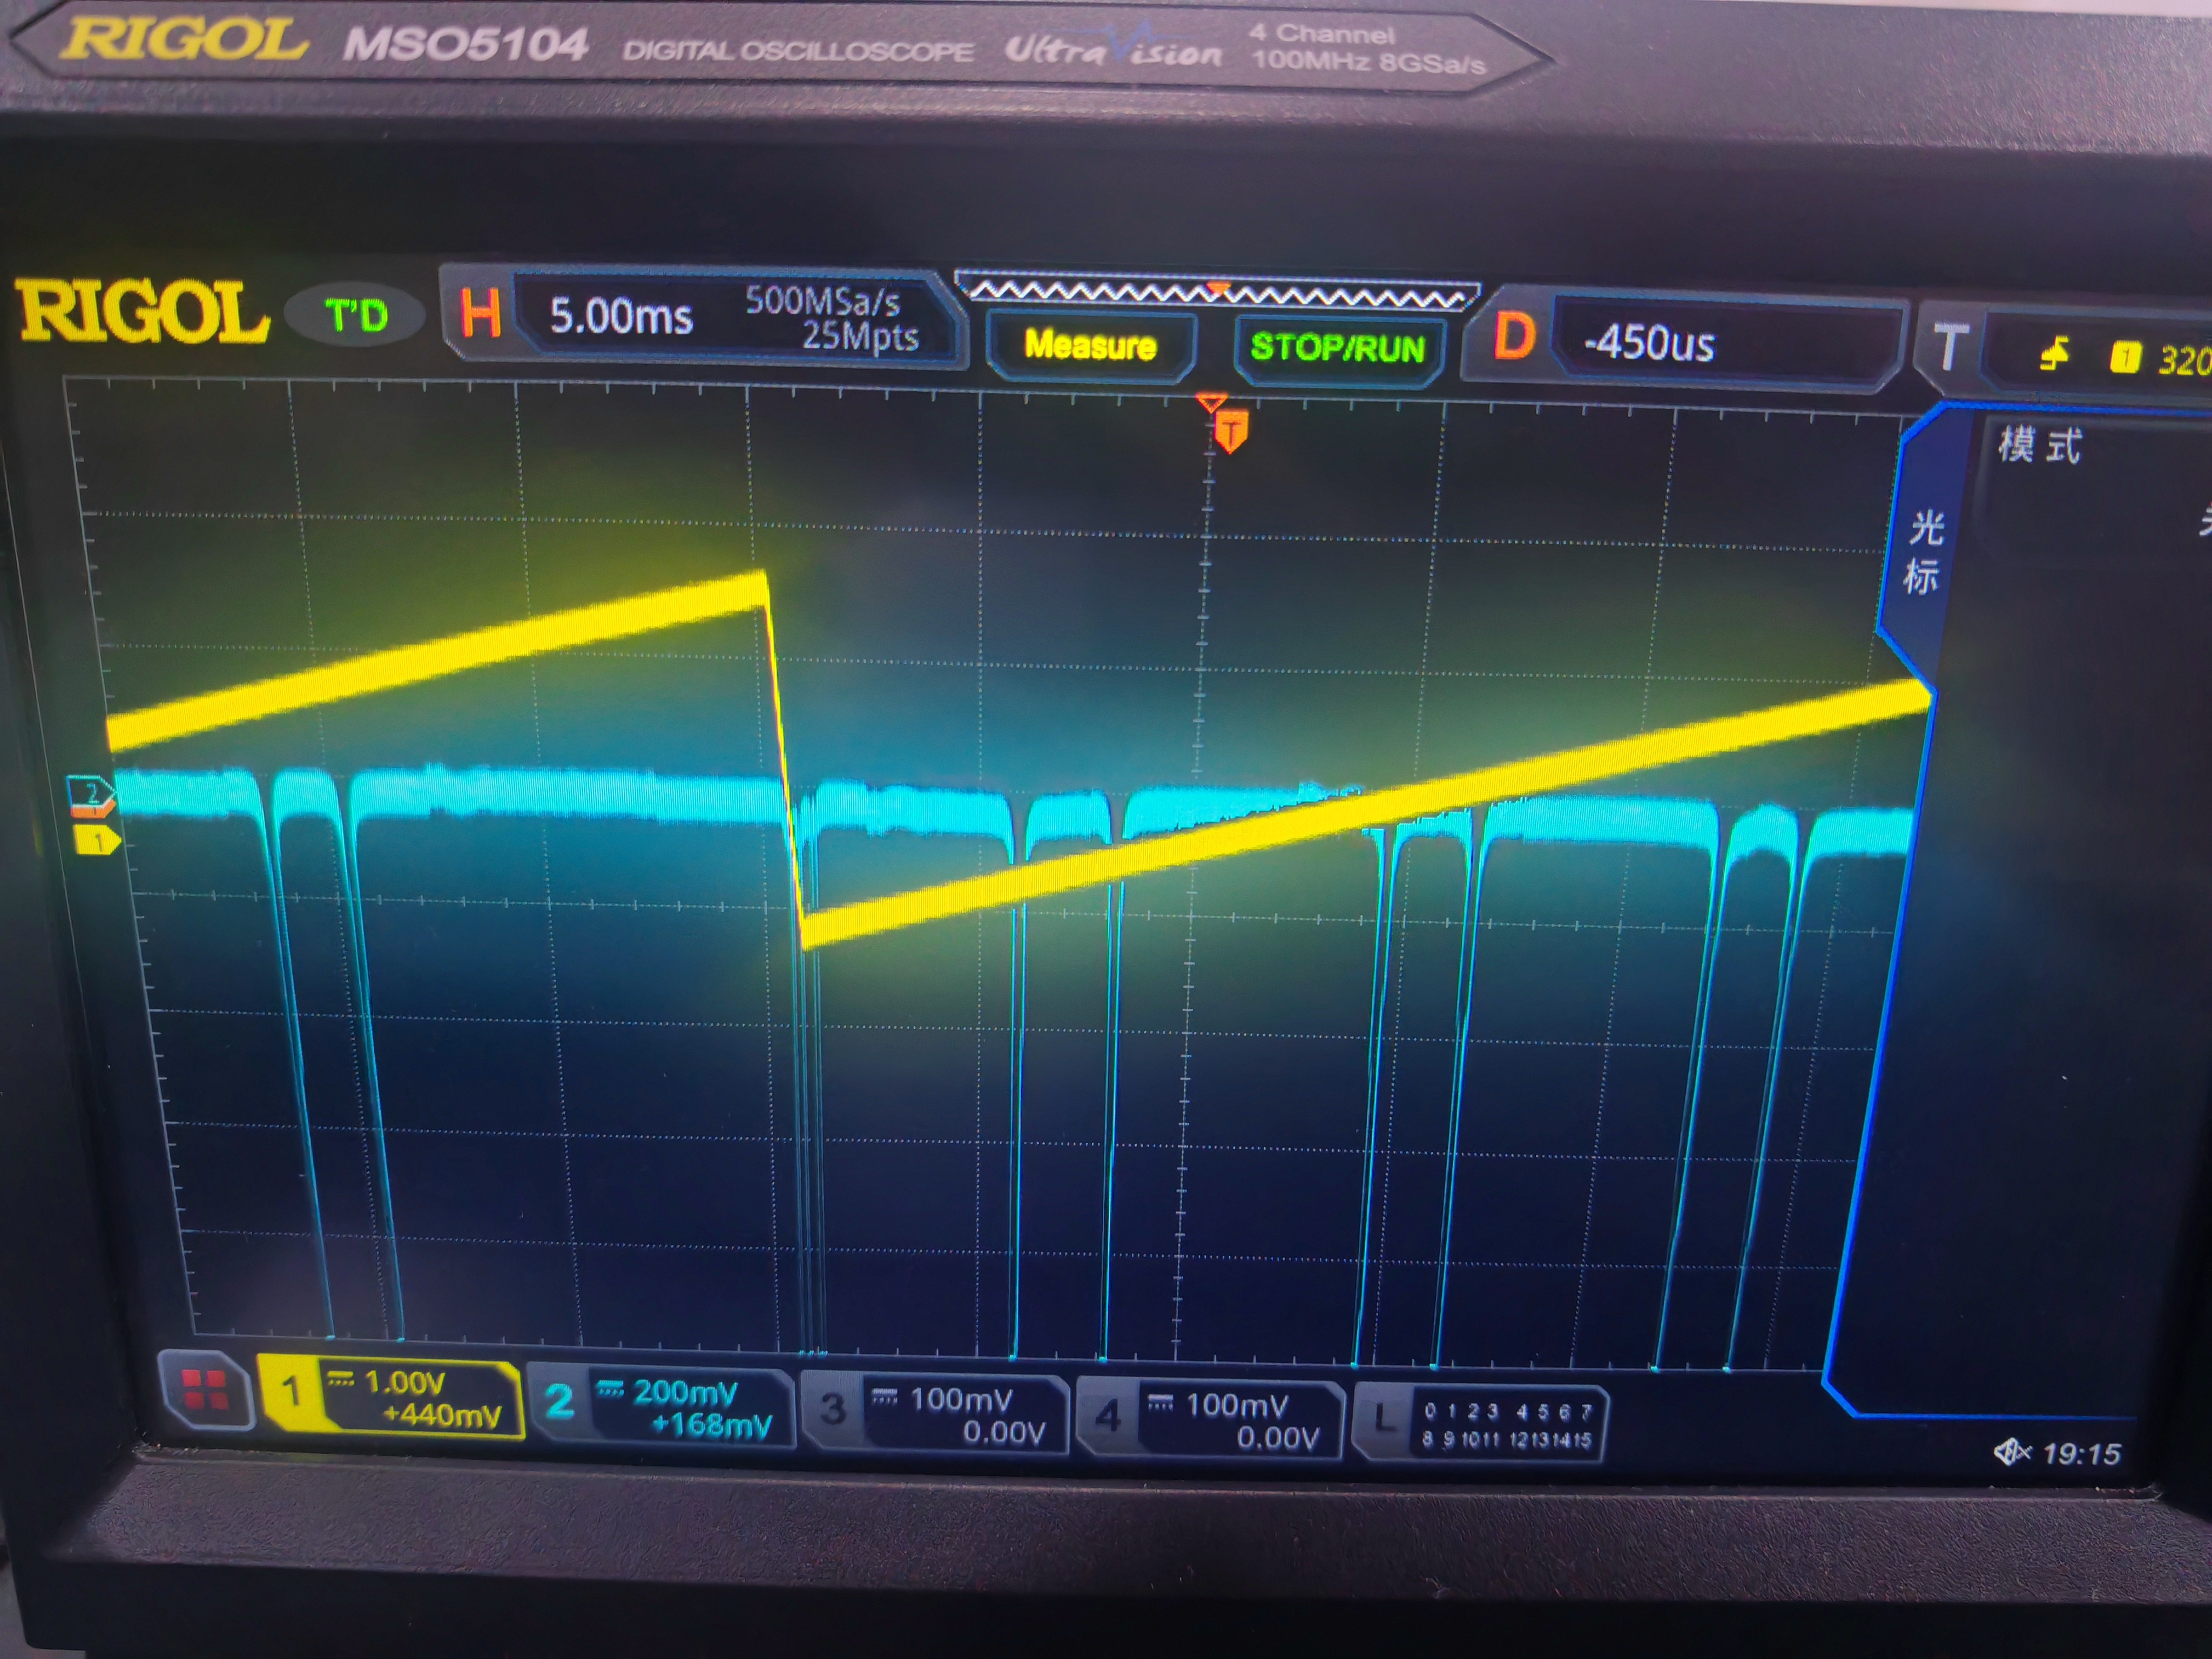
\includegraphics[width=\linewidth]{fig1.1.jpg}
    \subcaption{第一组扫描模谱}
    \label{fig:exp1-1}
  \end{subfigure}\hfill
  \begin{subfigure}[t]{0.485\textwidth}
    \centering
    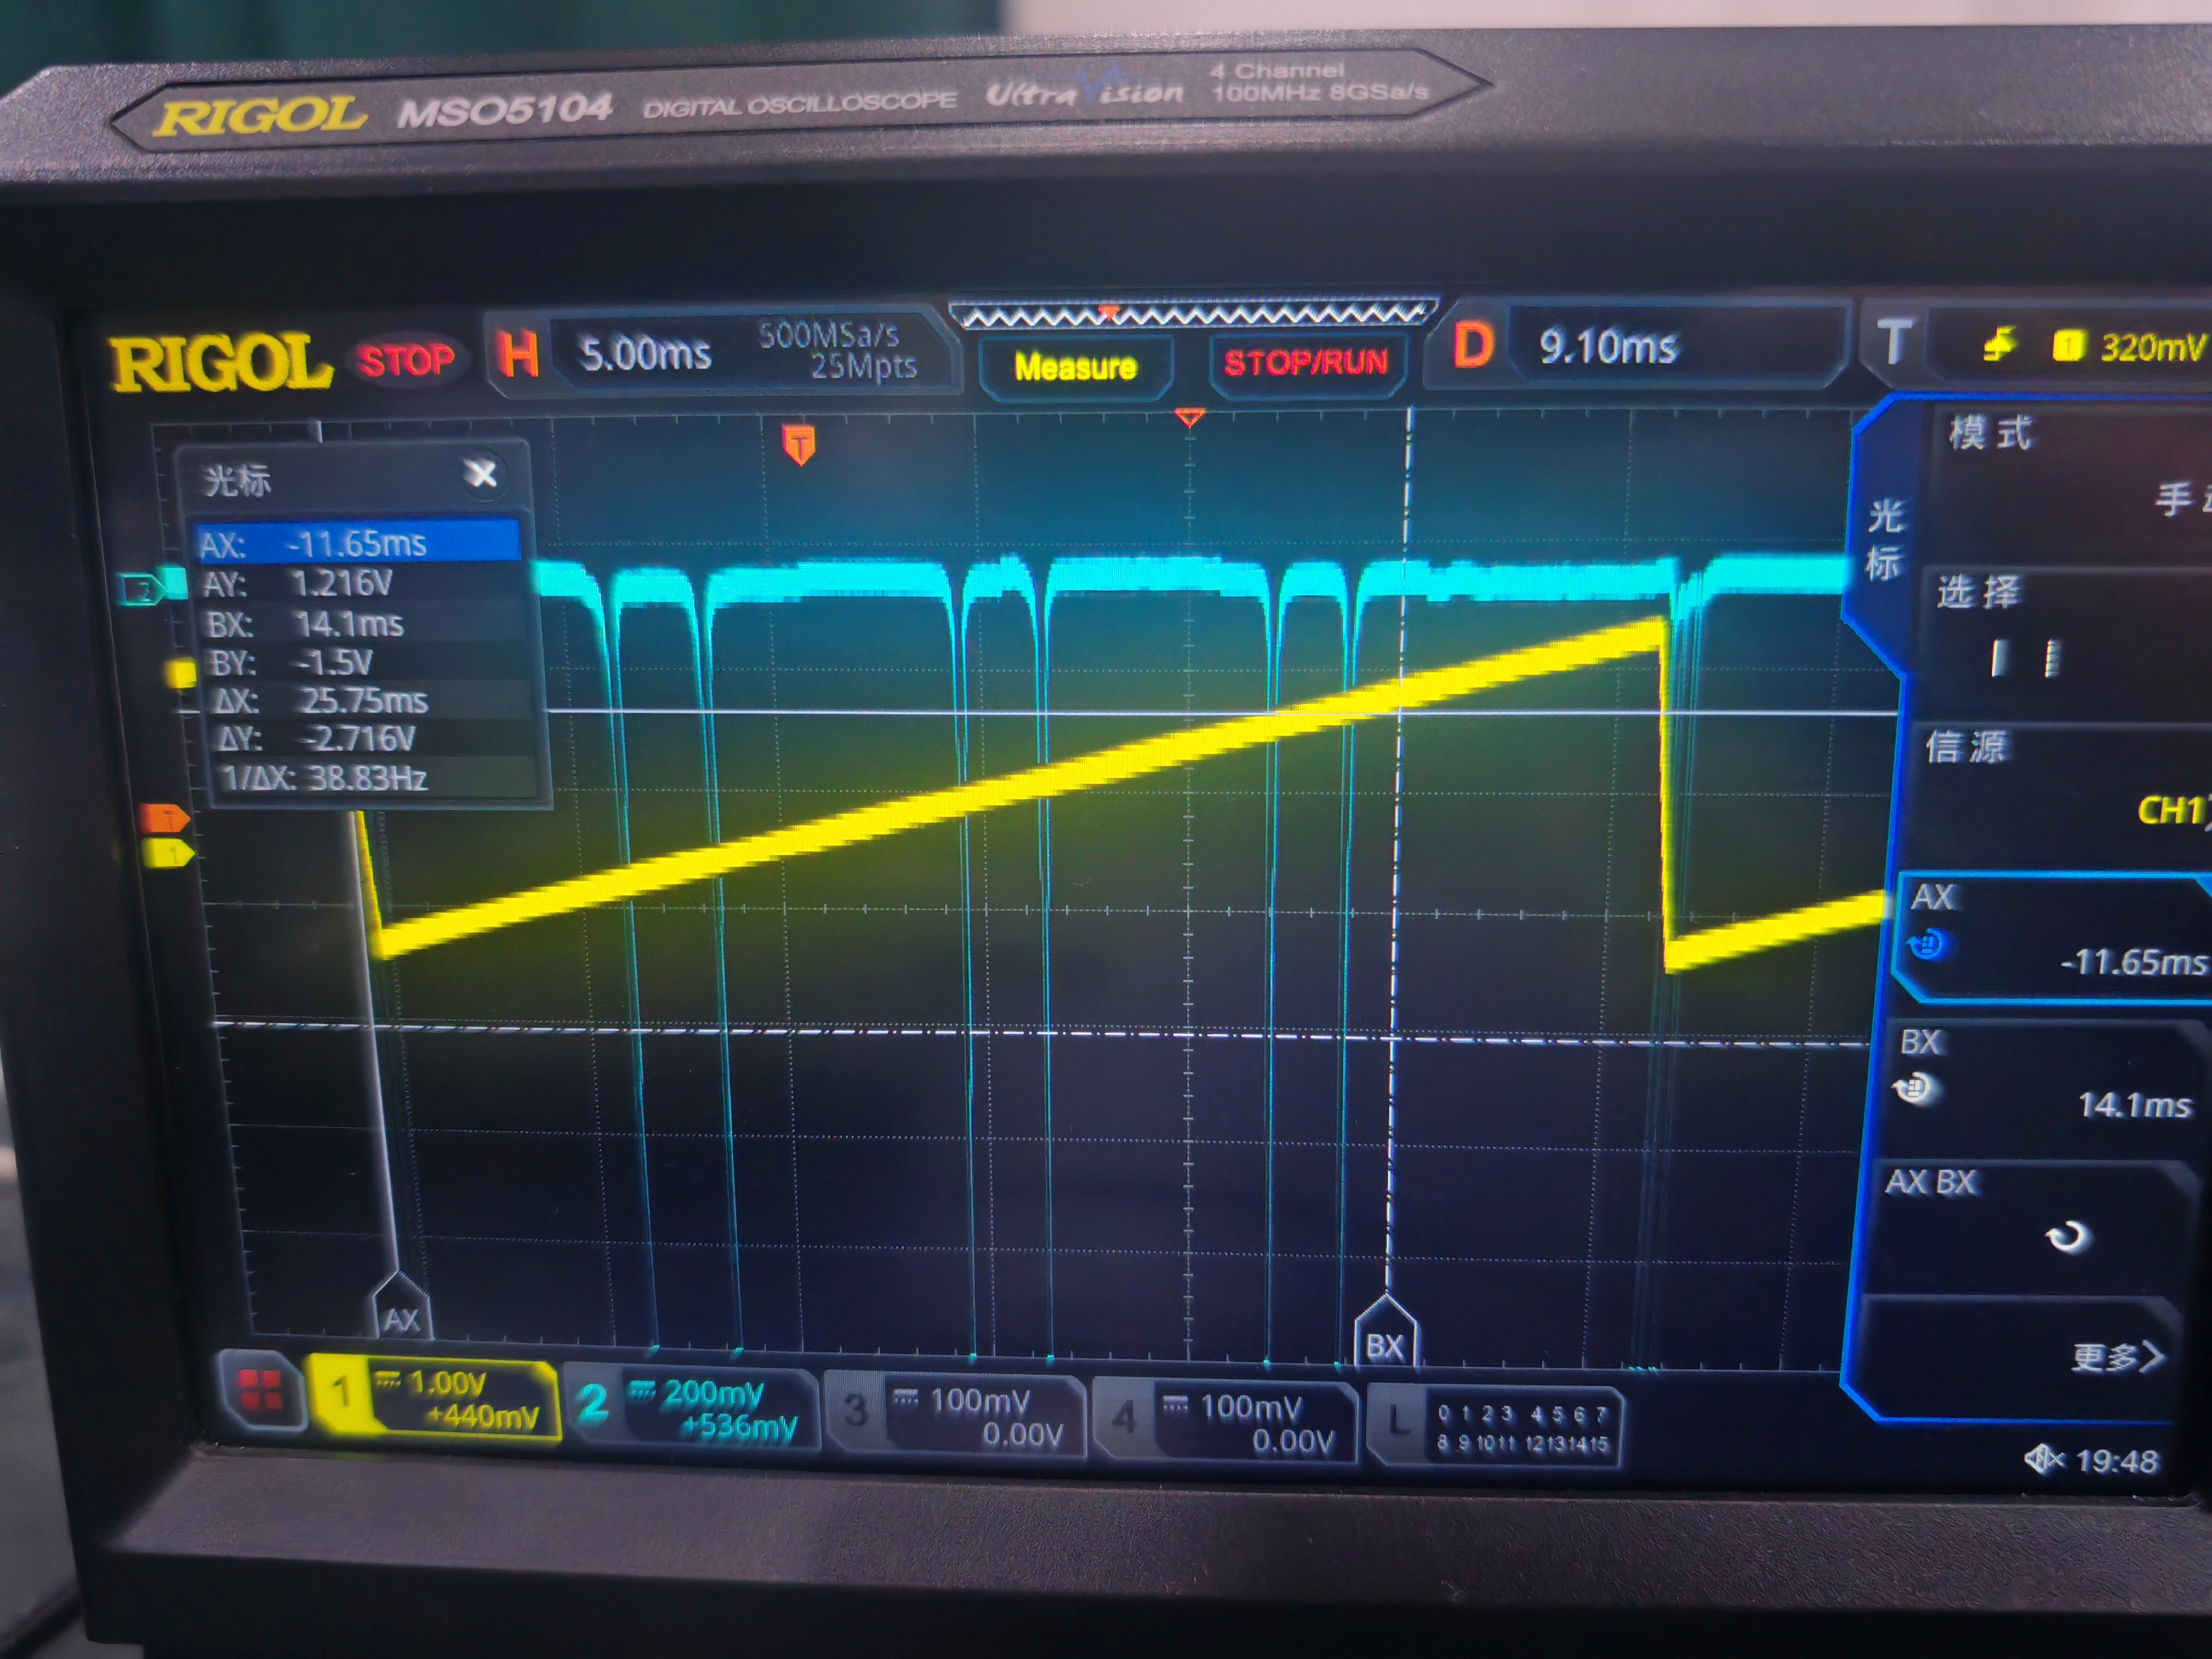
\includegraphics[width=\linewidth]{fig1.2.jpg}
    \subcaption{第二组扫描模谱及光标读数}
    \label{fig:exp1-2}
  \end{subfigure}
  \bicaption{单根 He-Ne 激光管管长测量的示波器记录。}{Oscilloscope records for measuring the cavity length of a single He-Ne laser tube.}
  \label{fig:exp1-scope}
\end{figure}

\begin{table}[H]
  \centering
  \caption{两组管长测量的时间间隔与频率换算}
  \label{tab:exp1-result}
  \begin{tabular}{ccccc}
    \toprule
    组次 & $\overline{\delta t}$/ms & $\overline{\delta T}$/ms & $\delta\nu$/MHz & 反算管长/mm \\
    \midrule
    1 & 2.0167 & 7.9125 & 679.74 & 220.7 \\
    2 & 1.9833 & 7.8250 & 675.98 & 221.9 \\
    \bottomrule
  \end{tabular}
\end{table}

以第一组为例，代入式\eqref{eq:scale}得到
\begin{equation}
  \delta\nu_1
  =\SI{2667}{\mega\hertz}\times
  \frac{\SI{2.0167}{\milli\second}}{\SI{7.9125}{\milli\second}}
  =\SI{679.74}{\mega\hertz}.
\end{equation}
第二组同理得到 $\delta\nu_2=\SI{675.98}{\mega\hertz}$，两组平均纵模频差为 \SI{677.86}{\mega\hertz}。取 $c=\SI{3.00e8}{\metre\per\second}$，由式\eqref{eq:tube-length}得到
\begin{equation}
  L=\frac{\SI{3.00e8}{\metre\per\second}}
  {2\times\SI{677.86e6}{\hertz}}
  =\SI{221.3}{\milli\metre}.
\end{equation}
该结果与尺量值 \SI{222}{\milli\metre} 相差 \SI{0.7}{\milli\metre}，相对偏差为 \SI{0.32}{\percent}。两组频差相差 \SI{3.76}{\mega\hertz}，说明重复测量一致性较好，主要偏差可能来自扫描轴非线性、峰位判读和有效腔长与外部尺量长度的差别。

\subsection{实验二：激光模式分析}

转动螺旋测微器时，观察屏上的光斑由基横模逐渐变为带一条节线的“8”字形分布，据此分别选定 $\mathrm{TEM}_{00}$ 和 $\mathrm{TEM}_{01}$ 工作状态。对应的示波器模谱见 Fig.~\ref{fig:exp2-scope}。$\mathrm{TEM}_{00}$ 数据按工作簿原有平均公式选取 \SI{1.55}{\milli\second} 和 \SI{1.35}{\milli\second} 两个间隔；照片与数据中的末端峰接近锯齿回扫区域，因此未将 \SI{1.25}{\milli\second} 纳入平均。$\mathrm{TEM}_{01}$ 状态则选取线性扫描段内三组清晰峰间距。

\begin{figure}[H]
  \centering
  \begin{subfigure}[t]{0.485\textwidth}
    \centering
    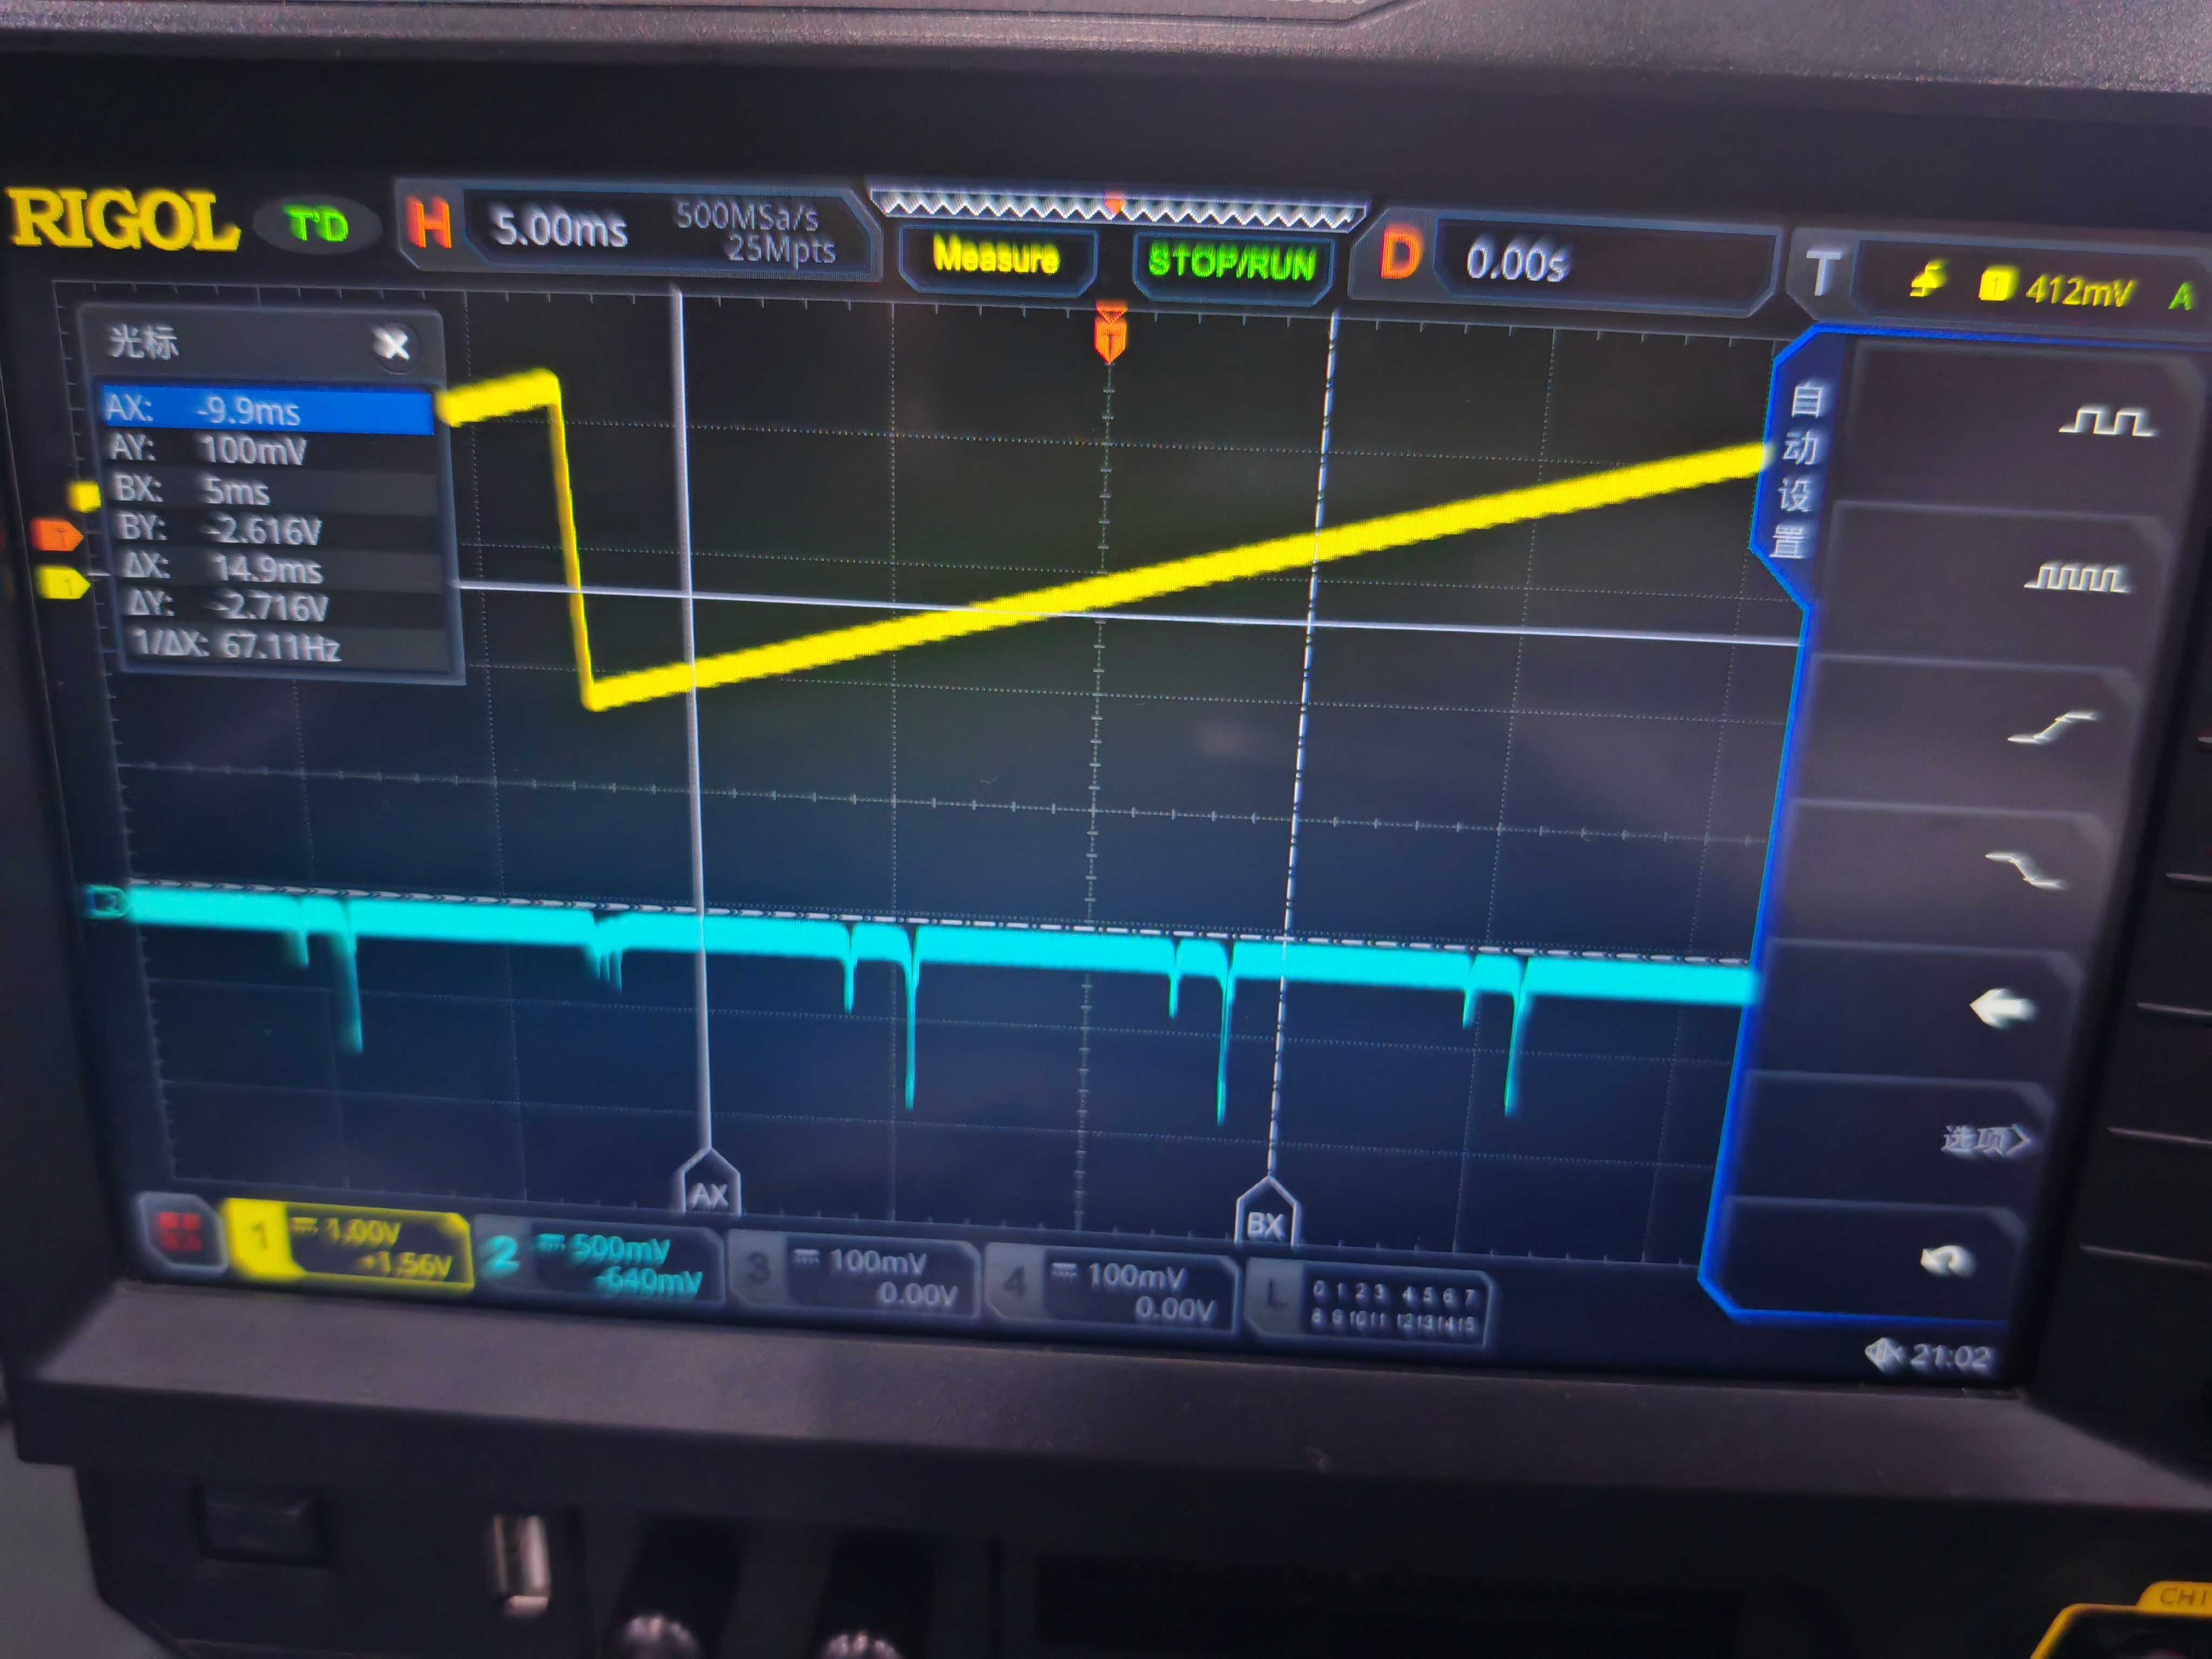
\includegraphics[width=\linewidth]{fig2.1(TEM00).jpg}
    \subcaption{$\mathrm{TEM}_{00}$ 状态的示波器模谱}
    \label{fig:exp2-tem00}
  \end{subfigure}\hfill
  \begin{subfigure}[t]{0.485\textwidth}
    \centering
    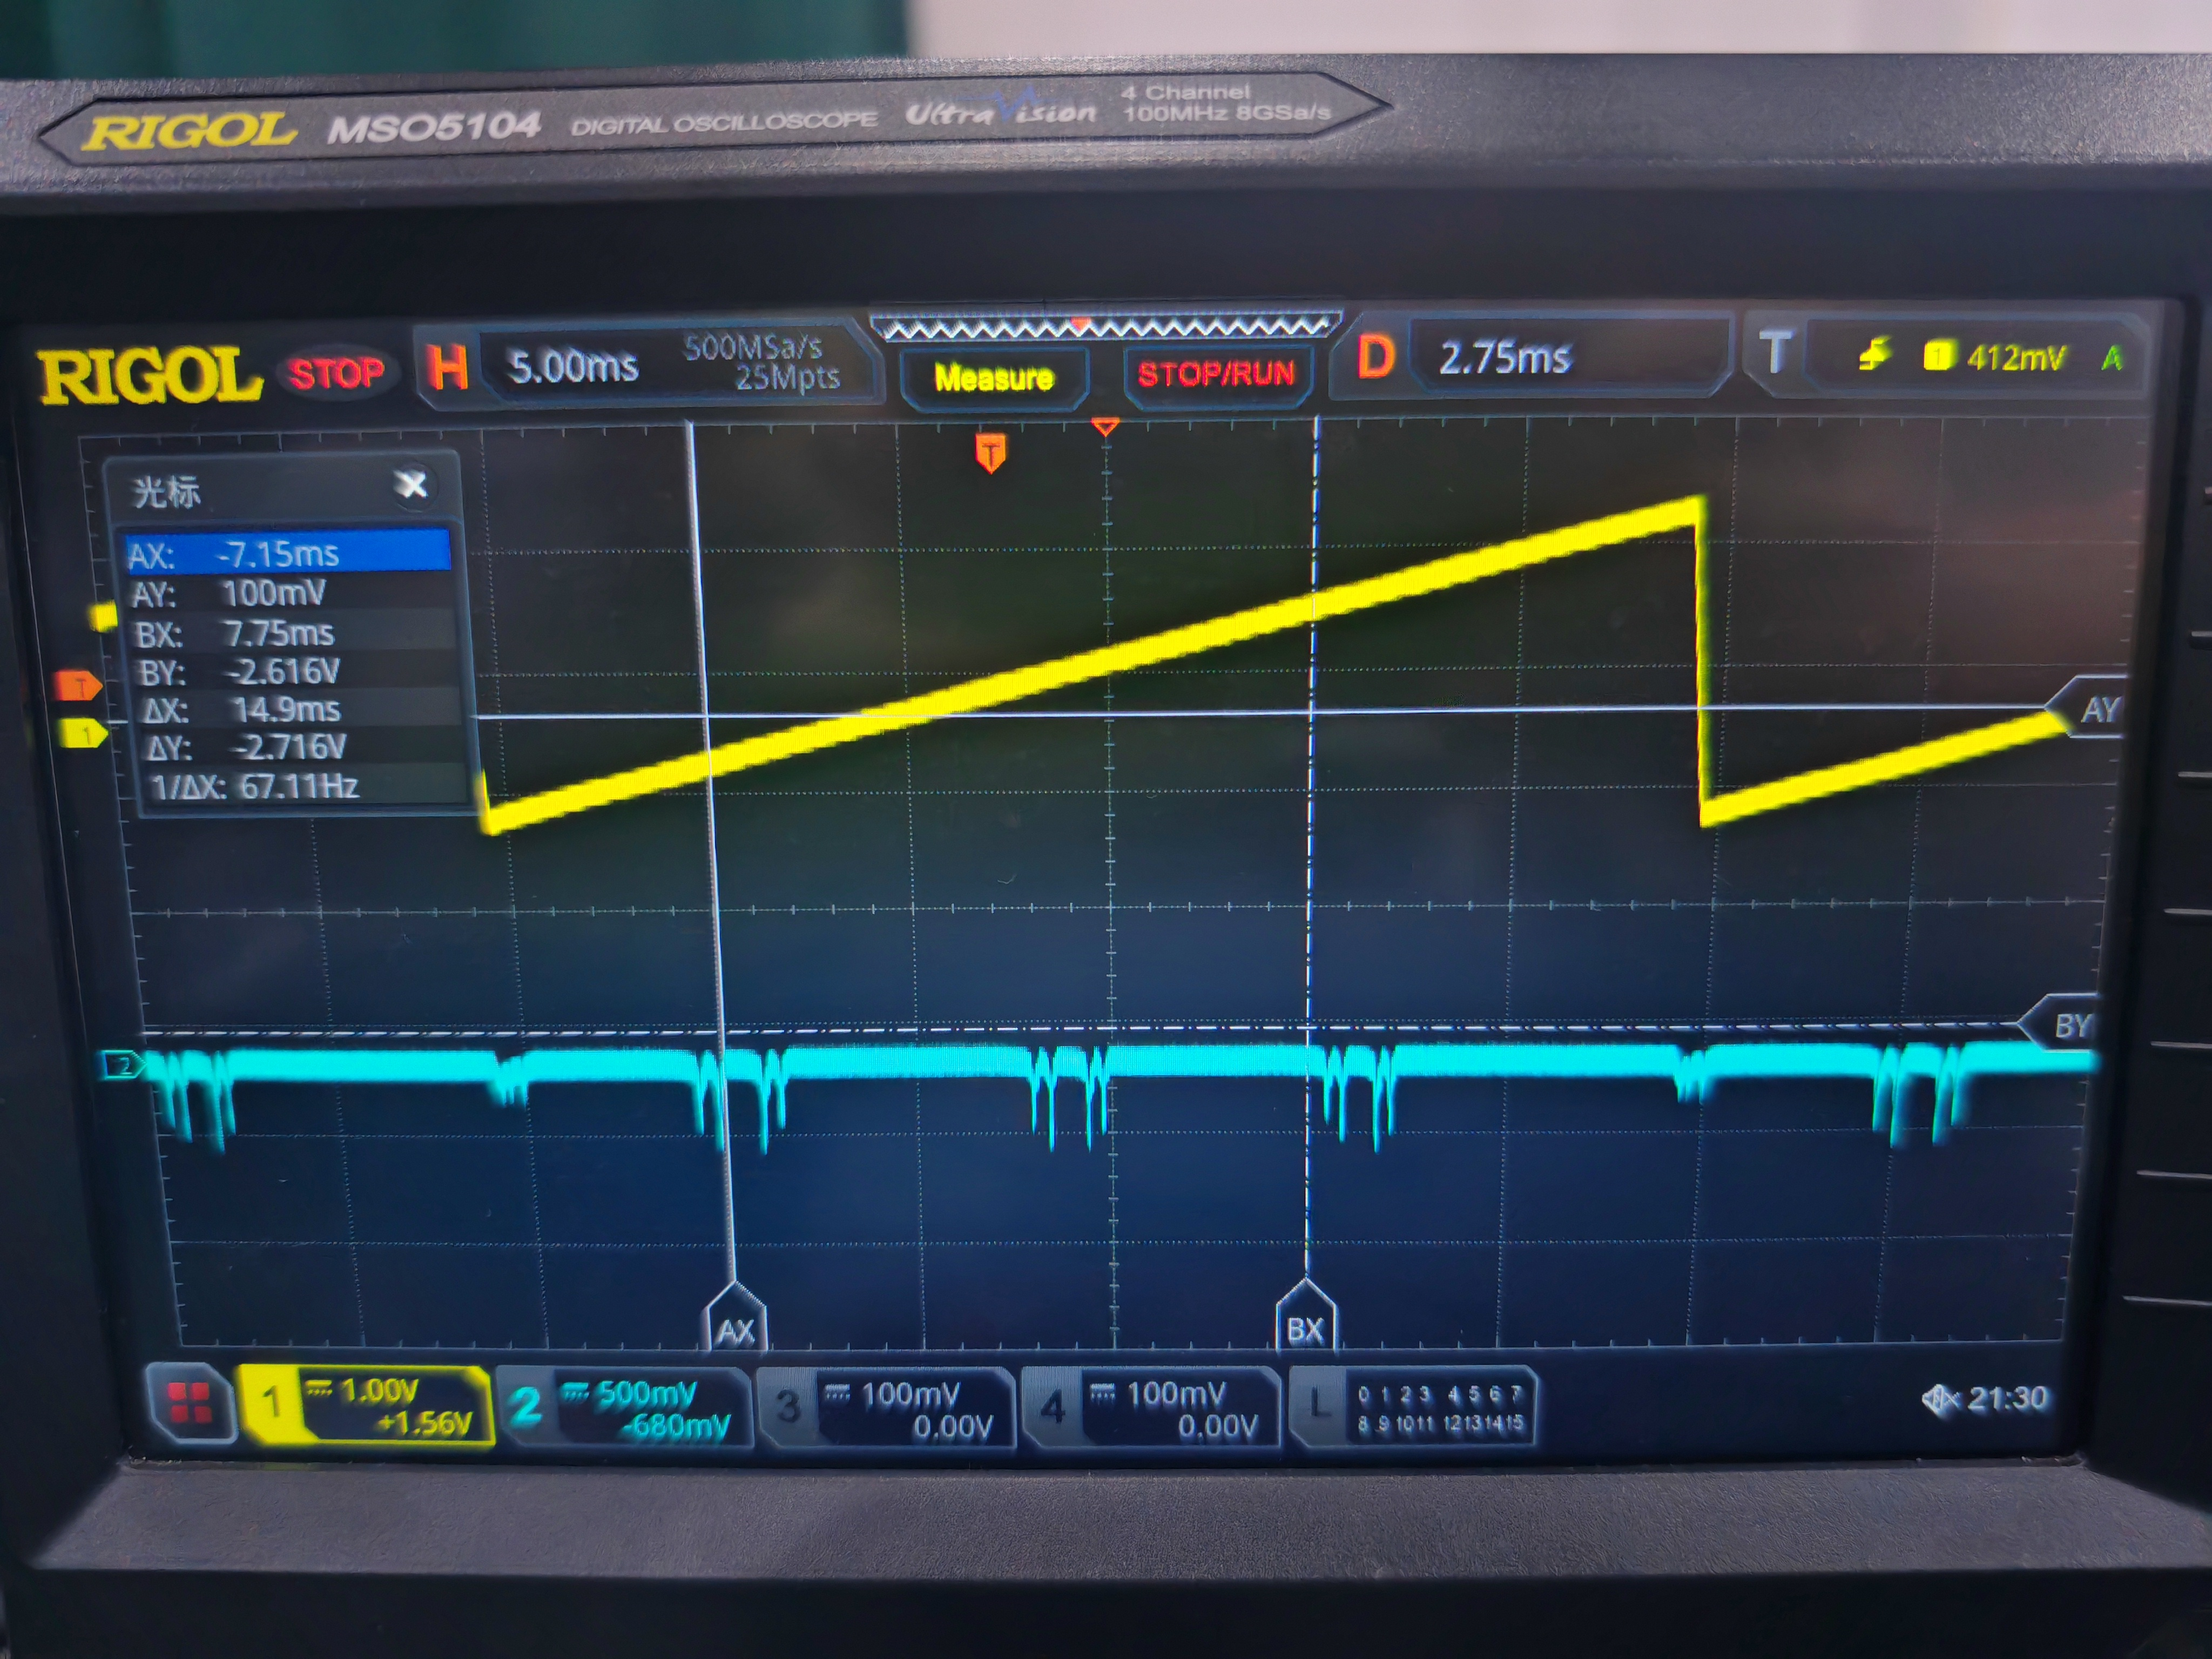
\includegraphics[width=\linewidth]{fig2.2(TEM01).jpg}
    \subcaption{$\mathrm{TEM}_{01}$ 状态的示波器模谱}
    \label{fig:exp2-tem01}
  \end{subfigure}
  \bicaption{螺旋测微器调节得到的两种横模状态；$\mathrm{TEM}_{01}$ 在观察屏上呈“8”字形光斑。}{Oscilloscope spectra of the two transverse-mode states selected by micrometer adjustment.}
  \label{fig:exp2-scope}
\end{figure}

\begin{table}[H]
  \centering
  \caption{激光模式分析的时间间隔与频率换算}
  \label{tab:exp2-result}
  \begin{tabular}{cccccc}
    \toprule
    模式状态 & 测量量 & $\delta t_i$/ms & $\overline{\delta t}$/ms & $\overline{\delta T}$/ms & $\delta\nu$/MHz \\
    \midrule
    $\mathrm{TEM}_{00}$ & 纵模 & 1.55, 1.35 & 1.4500 & 7.80 & 495.79 \\
    $\mathrm{TEM}_{01}$ & 横模 & 0.50, 0.45, 0.39 & 0.4467 & 7.90 & 150.79 \\
    $\mathrm{TEM}_{01}$ & 纵模 & 1.63, 1.40, 1.25 & 1.4267 & 7.90 & 481.64 \\
    \bottomrule
  \end{tabular}
\end{table}

由式\eqref{eq:scale}，$\mathrm{TEM}_{00}$ 状态的纵模频差为 \SI{495.79}{\mega\hertz}；$\mathrm{TEM}_{01}$ 状态的横模频差和纵模频差分别为
\begin{equation}
  \delta\nu_{\mathrm{trans}}=\SI{150.79}{\mega\hertz},\qquad
  \delta\nu_{\mathrm{long}}=\SI{481.64}{\mega\hertz}.
\end{equation}
两种状态所得纵模频差相差 \SI{14.15}{\mega\hertz}，相对其平均值 \SI{488.71}{\mega\hertz} 的差异为 \SI{2.90}{\percent}。两者数量级一致，差异可由螺旋测微器调节后腔长变化、模式跳变以及锯齿扫描非线性解释。横模频差明显小于纵模频差，且与观察屏上的 $\mathrm{TEM}_{01}$ “8”字形强度分布相互印证。

\subsection{实验三：出光带宽测量}

将示波器设为无限余辉并从小到大调节压电陶瓷电源后，屏幕上保留了多次扫描形成的宽带谱线。图\ref{fig:bandwidth-scope}给出了该状态下的示波器记录及测量量标注：$t_L$ 和 $t_R$ 分别为同一个宽带谱段的左、右边界，$\Delta t$ 为该谱段两边界的时间差，$T_{\mathrm{FSR}}$ 为从一个谱峰到下一个相邻谱峰的时间间隔。图\ref{fig:bandwidth-scope}中标出了同一宽带谱段的 $t_L$、$t_R$、边界间隔 $\Delta t=t_R-t_L$，以及从一个峰到下一个相邻峰的 $T_{\mathrm{FSR}}$。出光带宽的三次测量及频率换算结果见表\ref{tab:bandwidth-result}。其中 $t_R-t_L$ 为单个宽带谱段的时间宽度。以第 1 次测量为例，由式\eqref{eq:bandwidth}得到

\begin{figure}[H]
  \centering
  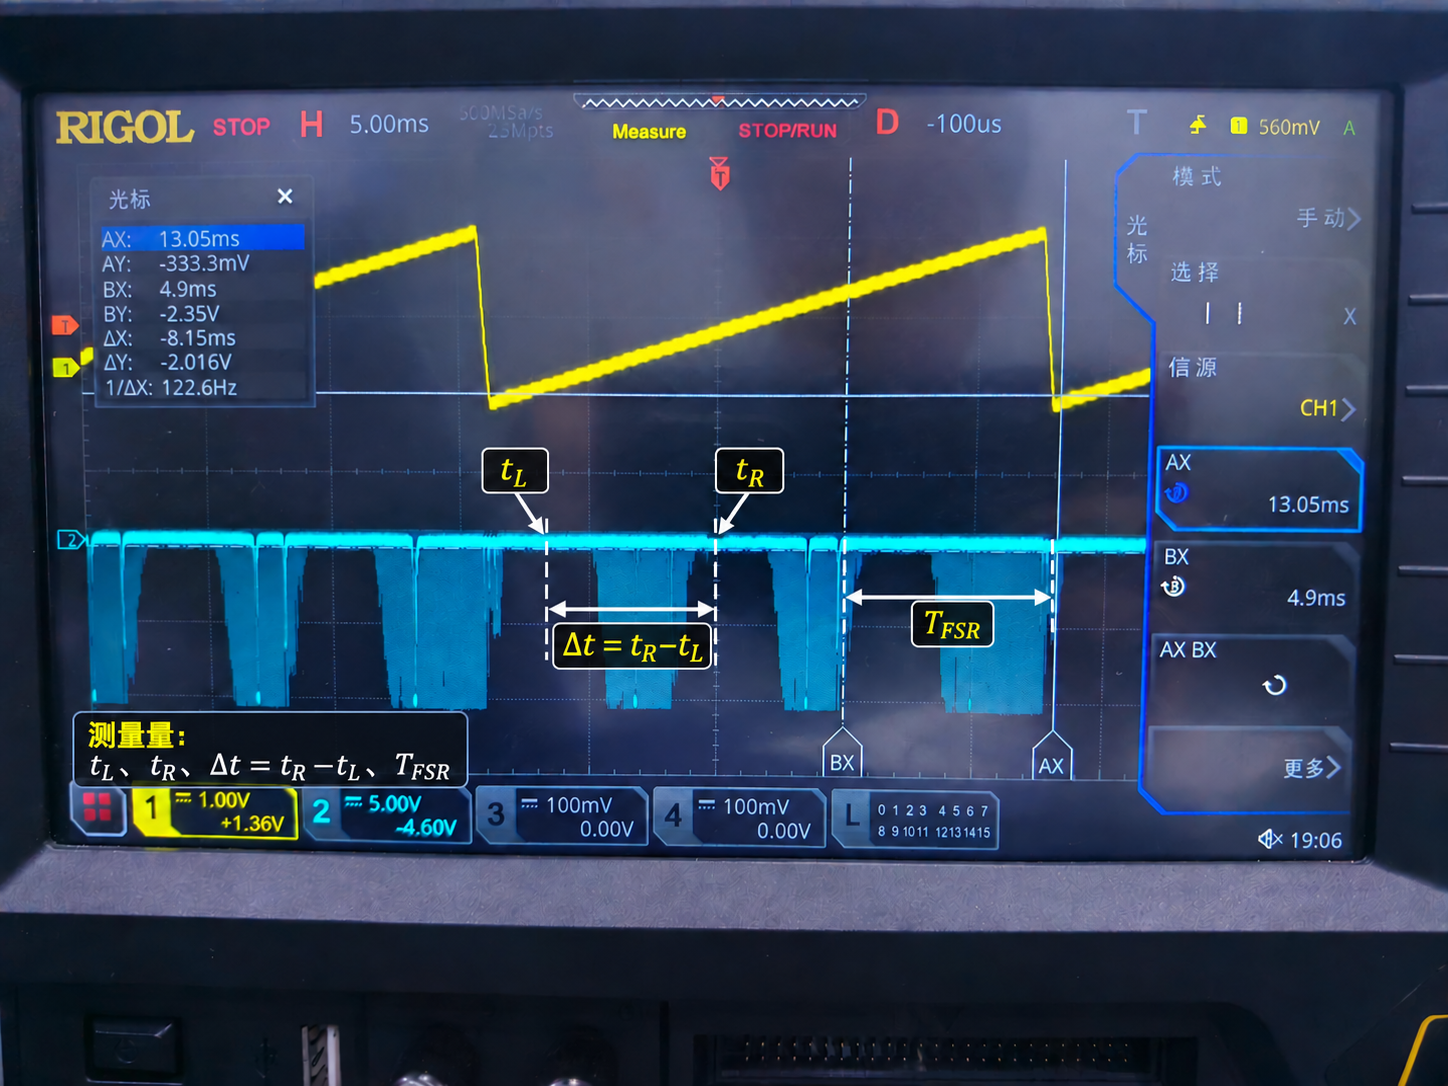
\includegraphics[width=0.8\textwidth]{fig3.1_bandwidth_annotated.png}
  \bicaption{无限余辉下出光带宽测量的示波器记录}{Oscilloscope record for the output bandwidth under infinite persistence}
  \label{fig:bandwidth-scope}
\end{figure}

 \begin{equation}
  \Delta\nu_{\mathrm{out},1}
  =\SI{2667}{\mega\hertz}\times
  \frac{\SI{2.70}{\milli\second}}{\SI{6.325}{\milli\second}}
  =\SI{1138.48}{\mega\hertz}.
\end{equation}

\begin{table}[H]
  \centering
  \caption{三次出光带宽测量与频率换算}
  \label{tab:bandwidth-result}
  \begin{tabular}{ccccccc}
    \toprule
    次数 & $t_R$/ms & $t_L$/ms & $t_R-t_L$/ms & $T_{\mathrm{FSR}}$/ms & $\nu_{\mathrm{FSR}}$/MHz & $\Delta\nu_{\mathrm{out}}$/MHz \\
    \midrule
    1 & -0.90 & -3.60 & 2.70 & 6.325 & 2667 & 1138.48 \\
    2 & 4.55 & 2.05 & 2.50 & 6.325 & 2667 & 1054.15 \\
    3 & -17.25 & -19.90 & 2.65 & 6.325 & 2667 & 1117.40 \\
    \midrule
    平均 & -- & -- & -- & -- & -- & 1103.34 \\
    \bottomrule
  \end{tabular}
\end{table}

三次测量的平均出光带宽为 \SI{1103.34}{\mega\hertz}，样本标准差为 \SI{43.89}{\mega\hertz}，标准误为 \SI{25.34}{\mega\hertz}，相对样本标准差为 \SI{3.98}{\percent}。三次结果的离散程度主要反映了左右边界峰判定和扫描时间轴读数的波动。

\subsection{实验四：分裂双峰的偏振关系}

固定石英晶片并旋转偏振片所得的四个典型状态见 Fig.~\ref{fig:polarization-scope}。图中两个分裂谱峰的高度随偏振片转角发生互补变化；由于示波器通道使峰形向下，原始电位为负，以下以峰值幅度 $U_i=|V_i|$ 进行处理。$0^\circ$、$90^\circ$、$180^\circ$ 和 $270^\circ$ 图像分别用于展示偏振片转角的代表性状态，其中 $270^\circ$ 与 $90^\circ$ 在理想线偏振片下具有相同的方向周期。

\begin{figure}[H]
  \centering
  \begin{subfigure}[t]{0.485\textwidth}
    \centering
    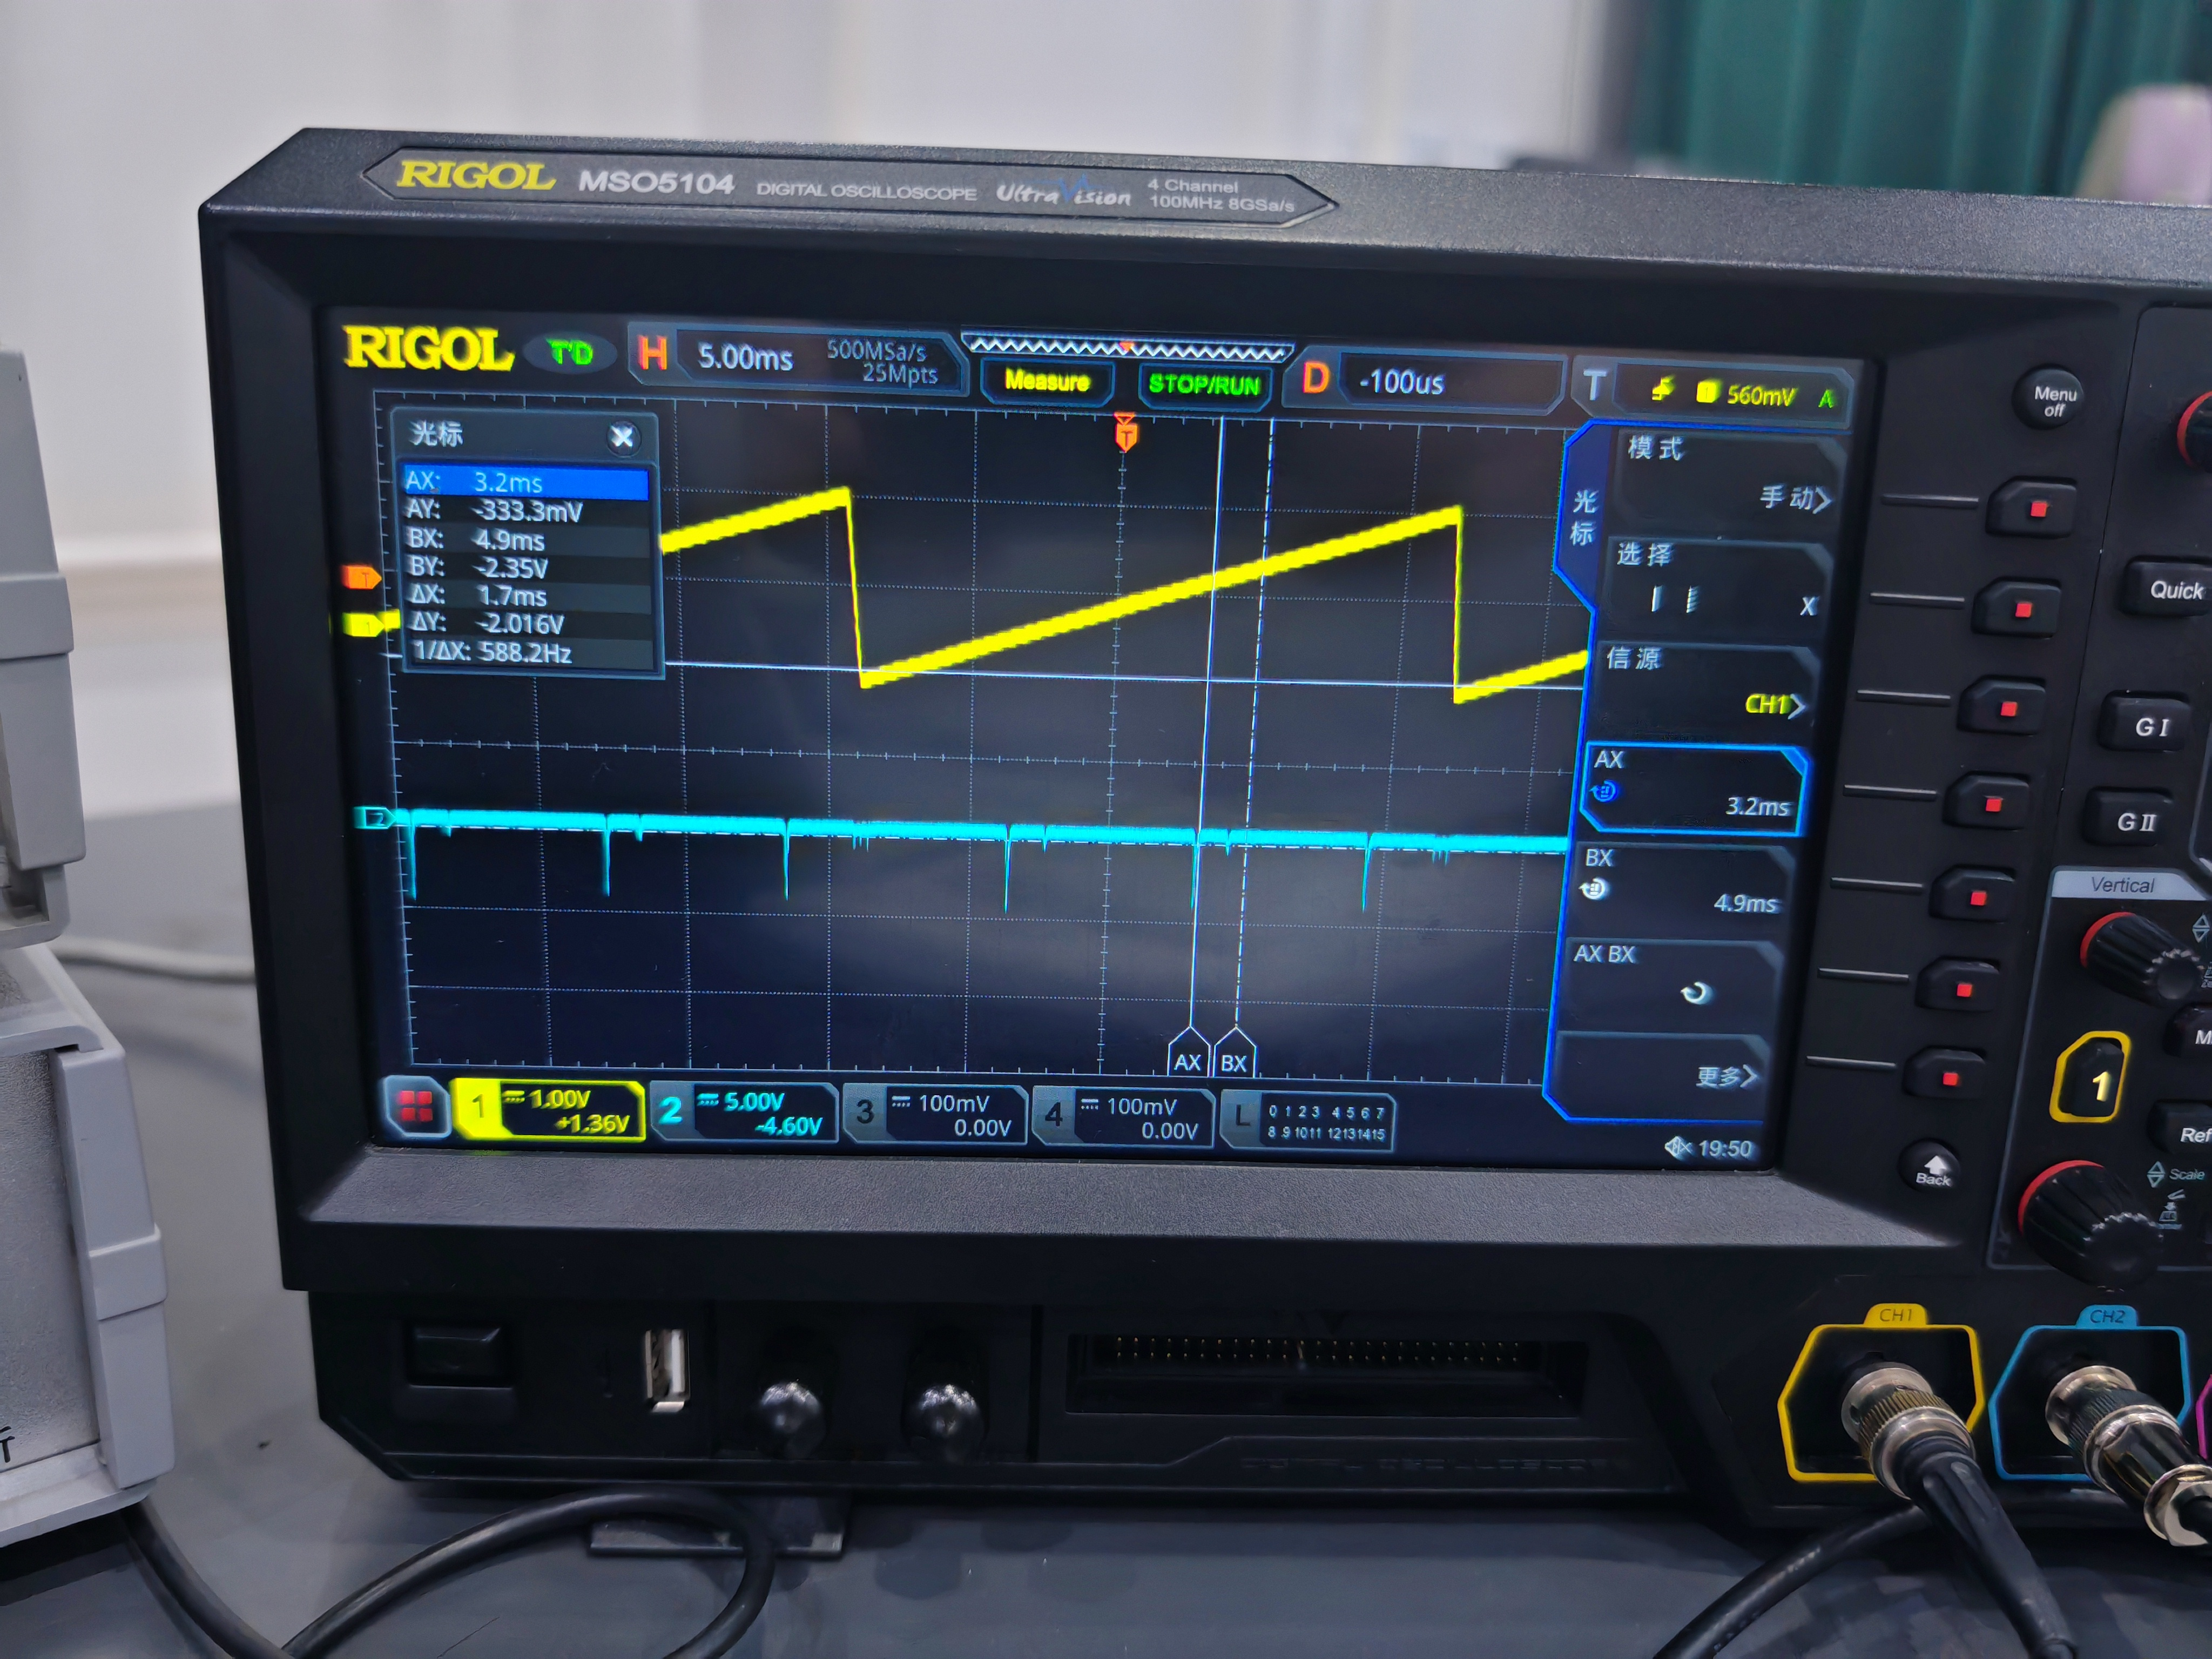
\includegraphics[width=\linewidth]{fig4.1_polarization_0.jpg}
    \subcaption{偏振片 $0^\circ$}
  \end{subfigure}\hfill
  \begin{subfigure}[t]{0.485\textwidth}
    \centering
    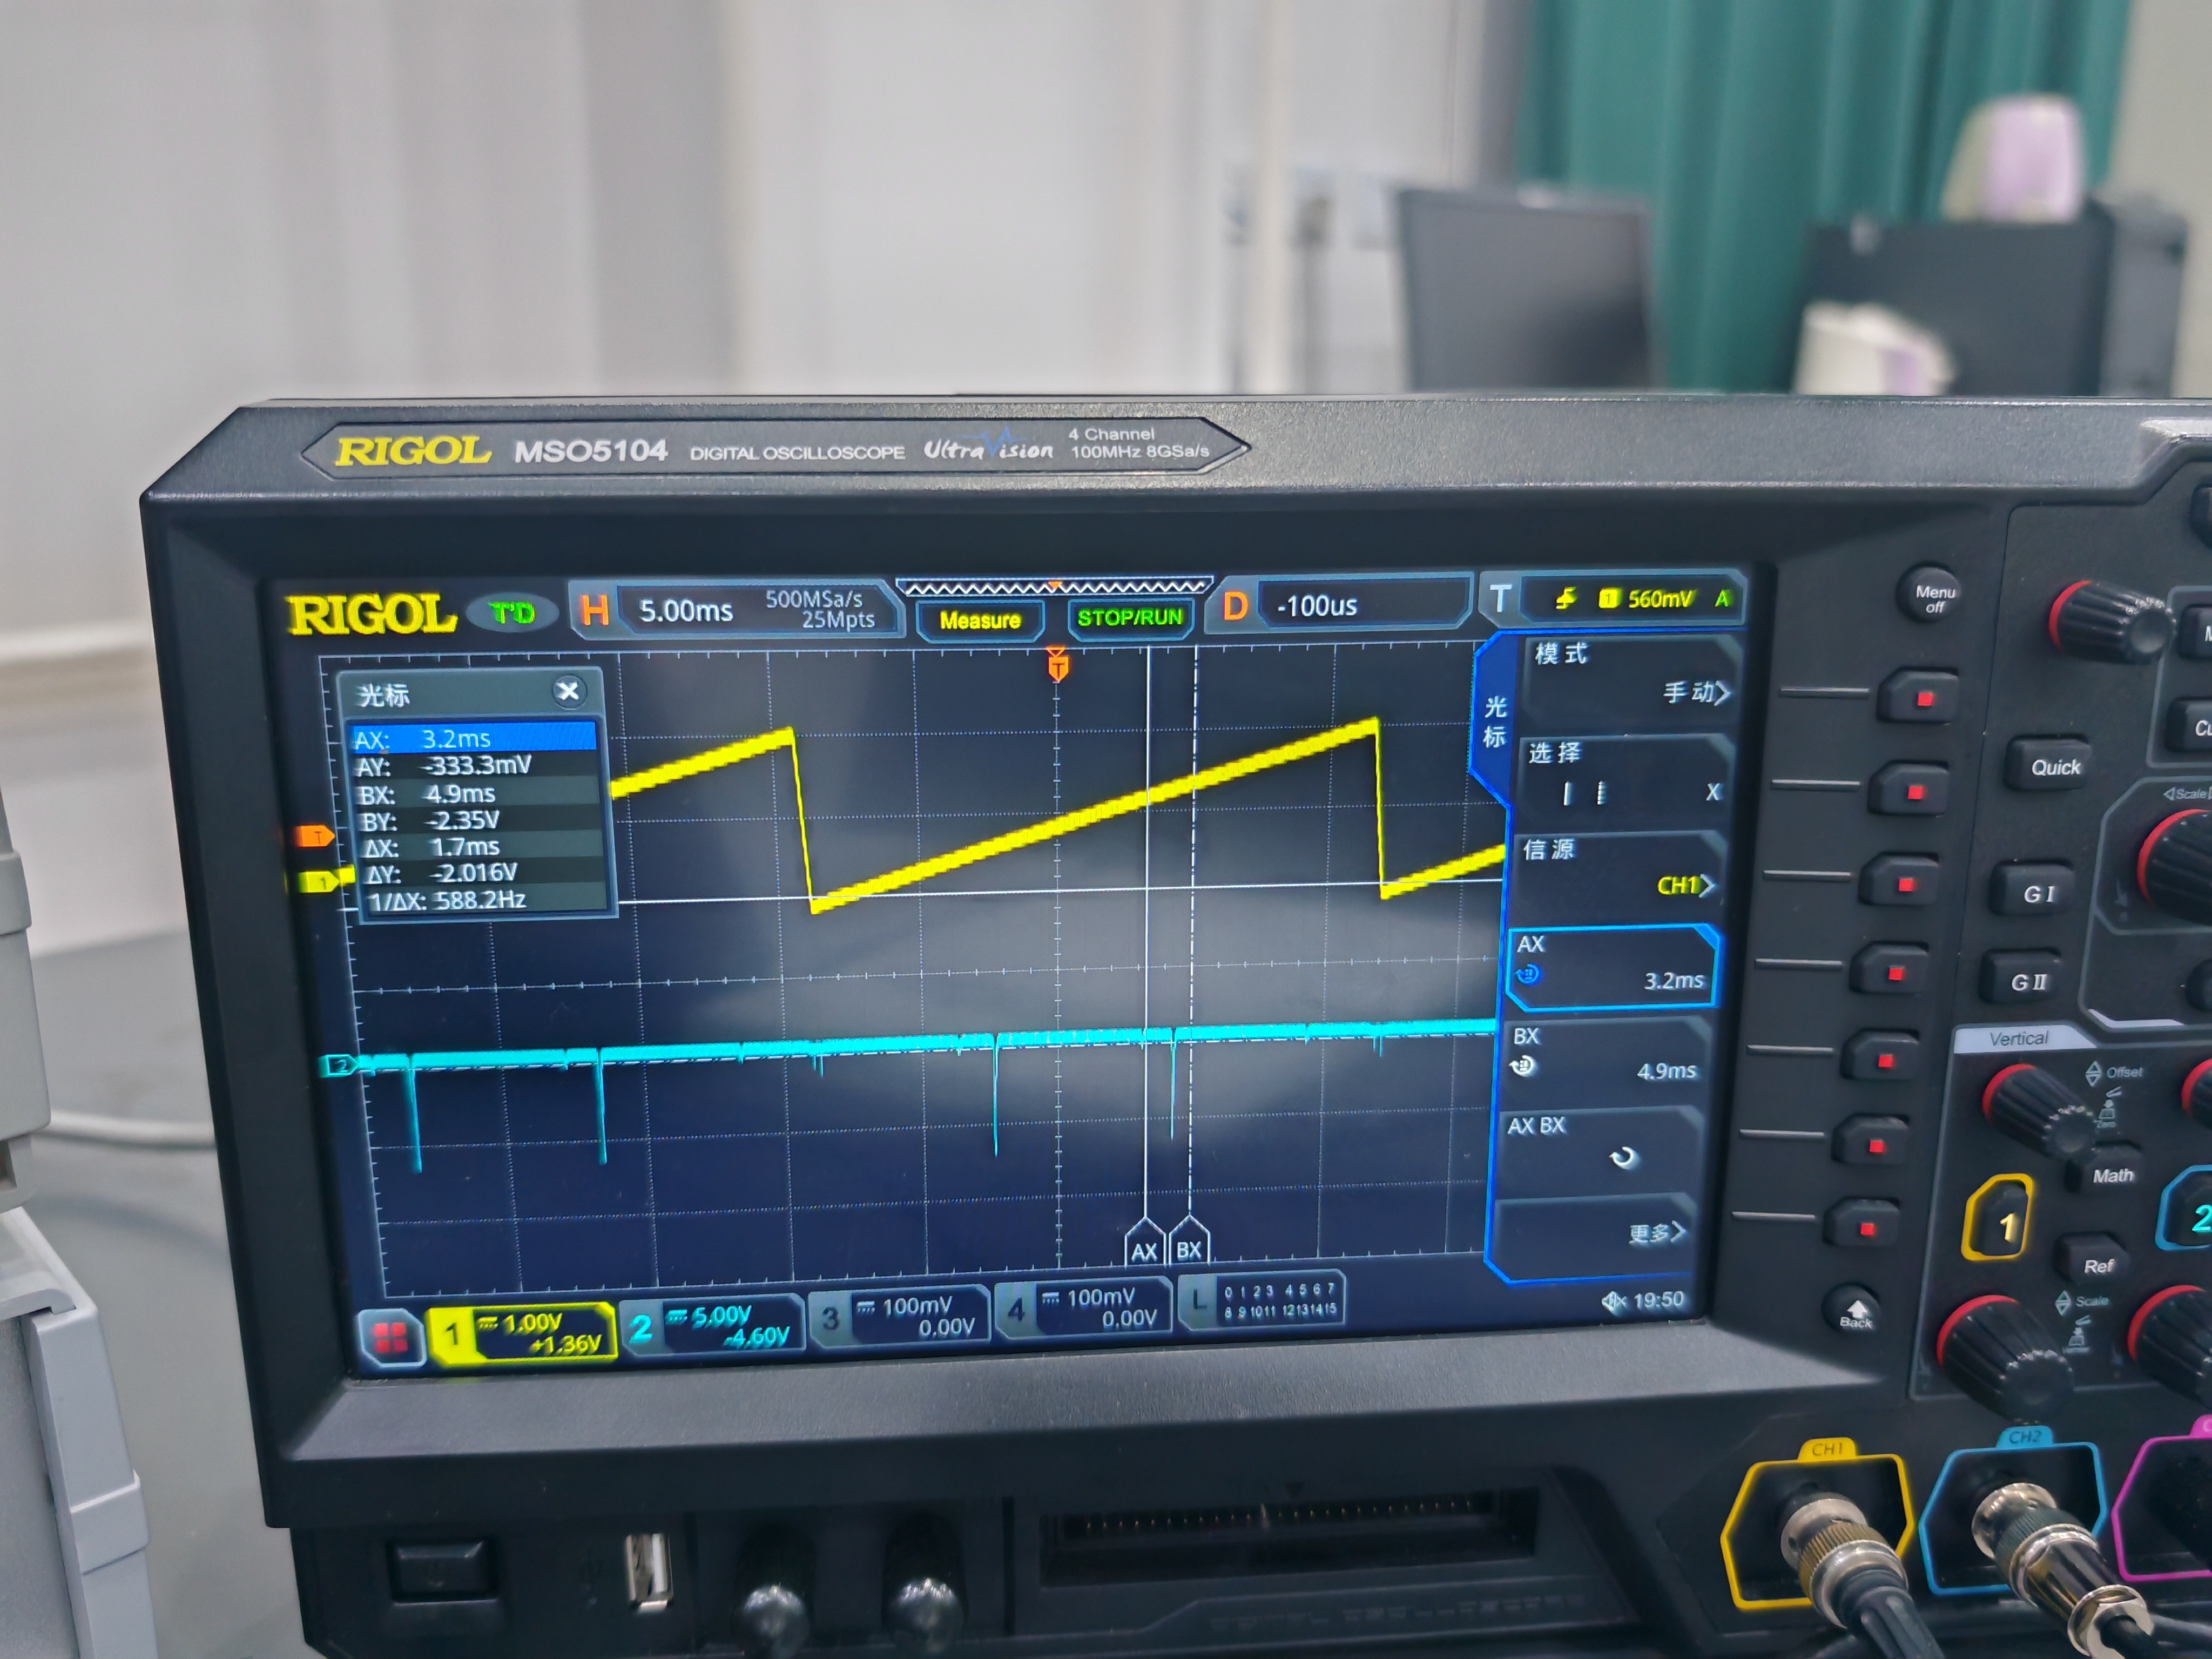
\includegraphics[width=\linewidth]{fig4.2_polarization_90.jpg}
    \subcaption{偏振片 $90^\circ$}
  \end{subfigure}

  \par\medskip
  \begin{subfigure}[t]{0.485\textwidth}
    \centering
    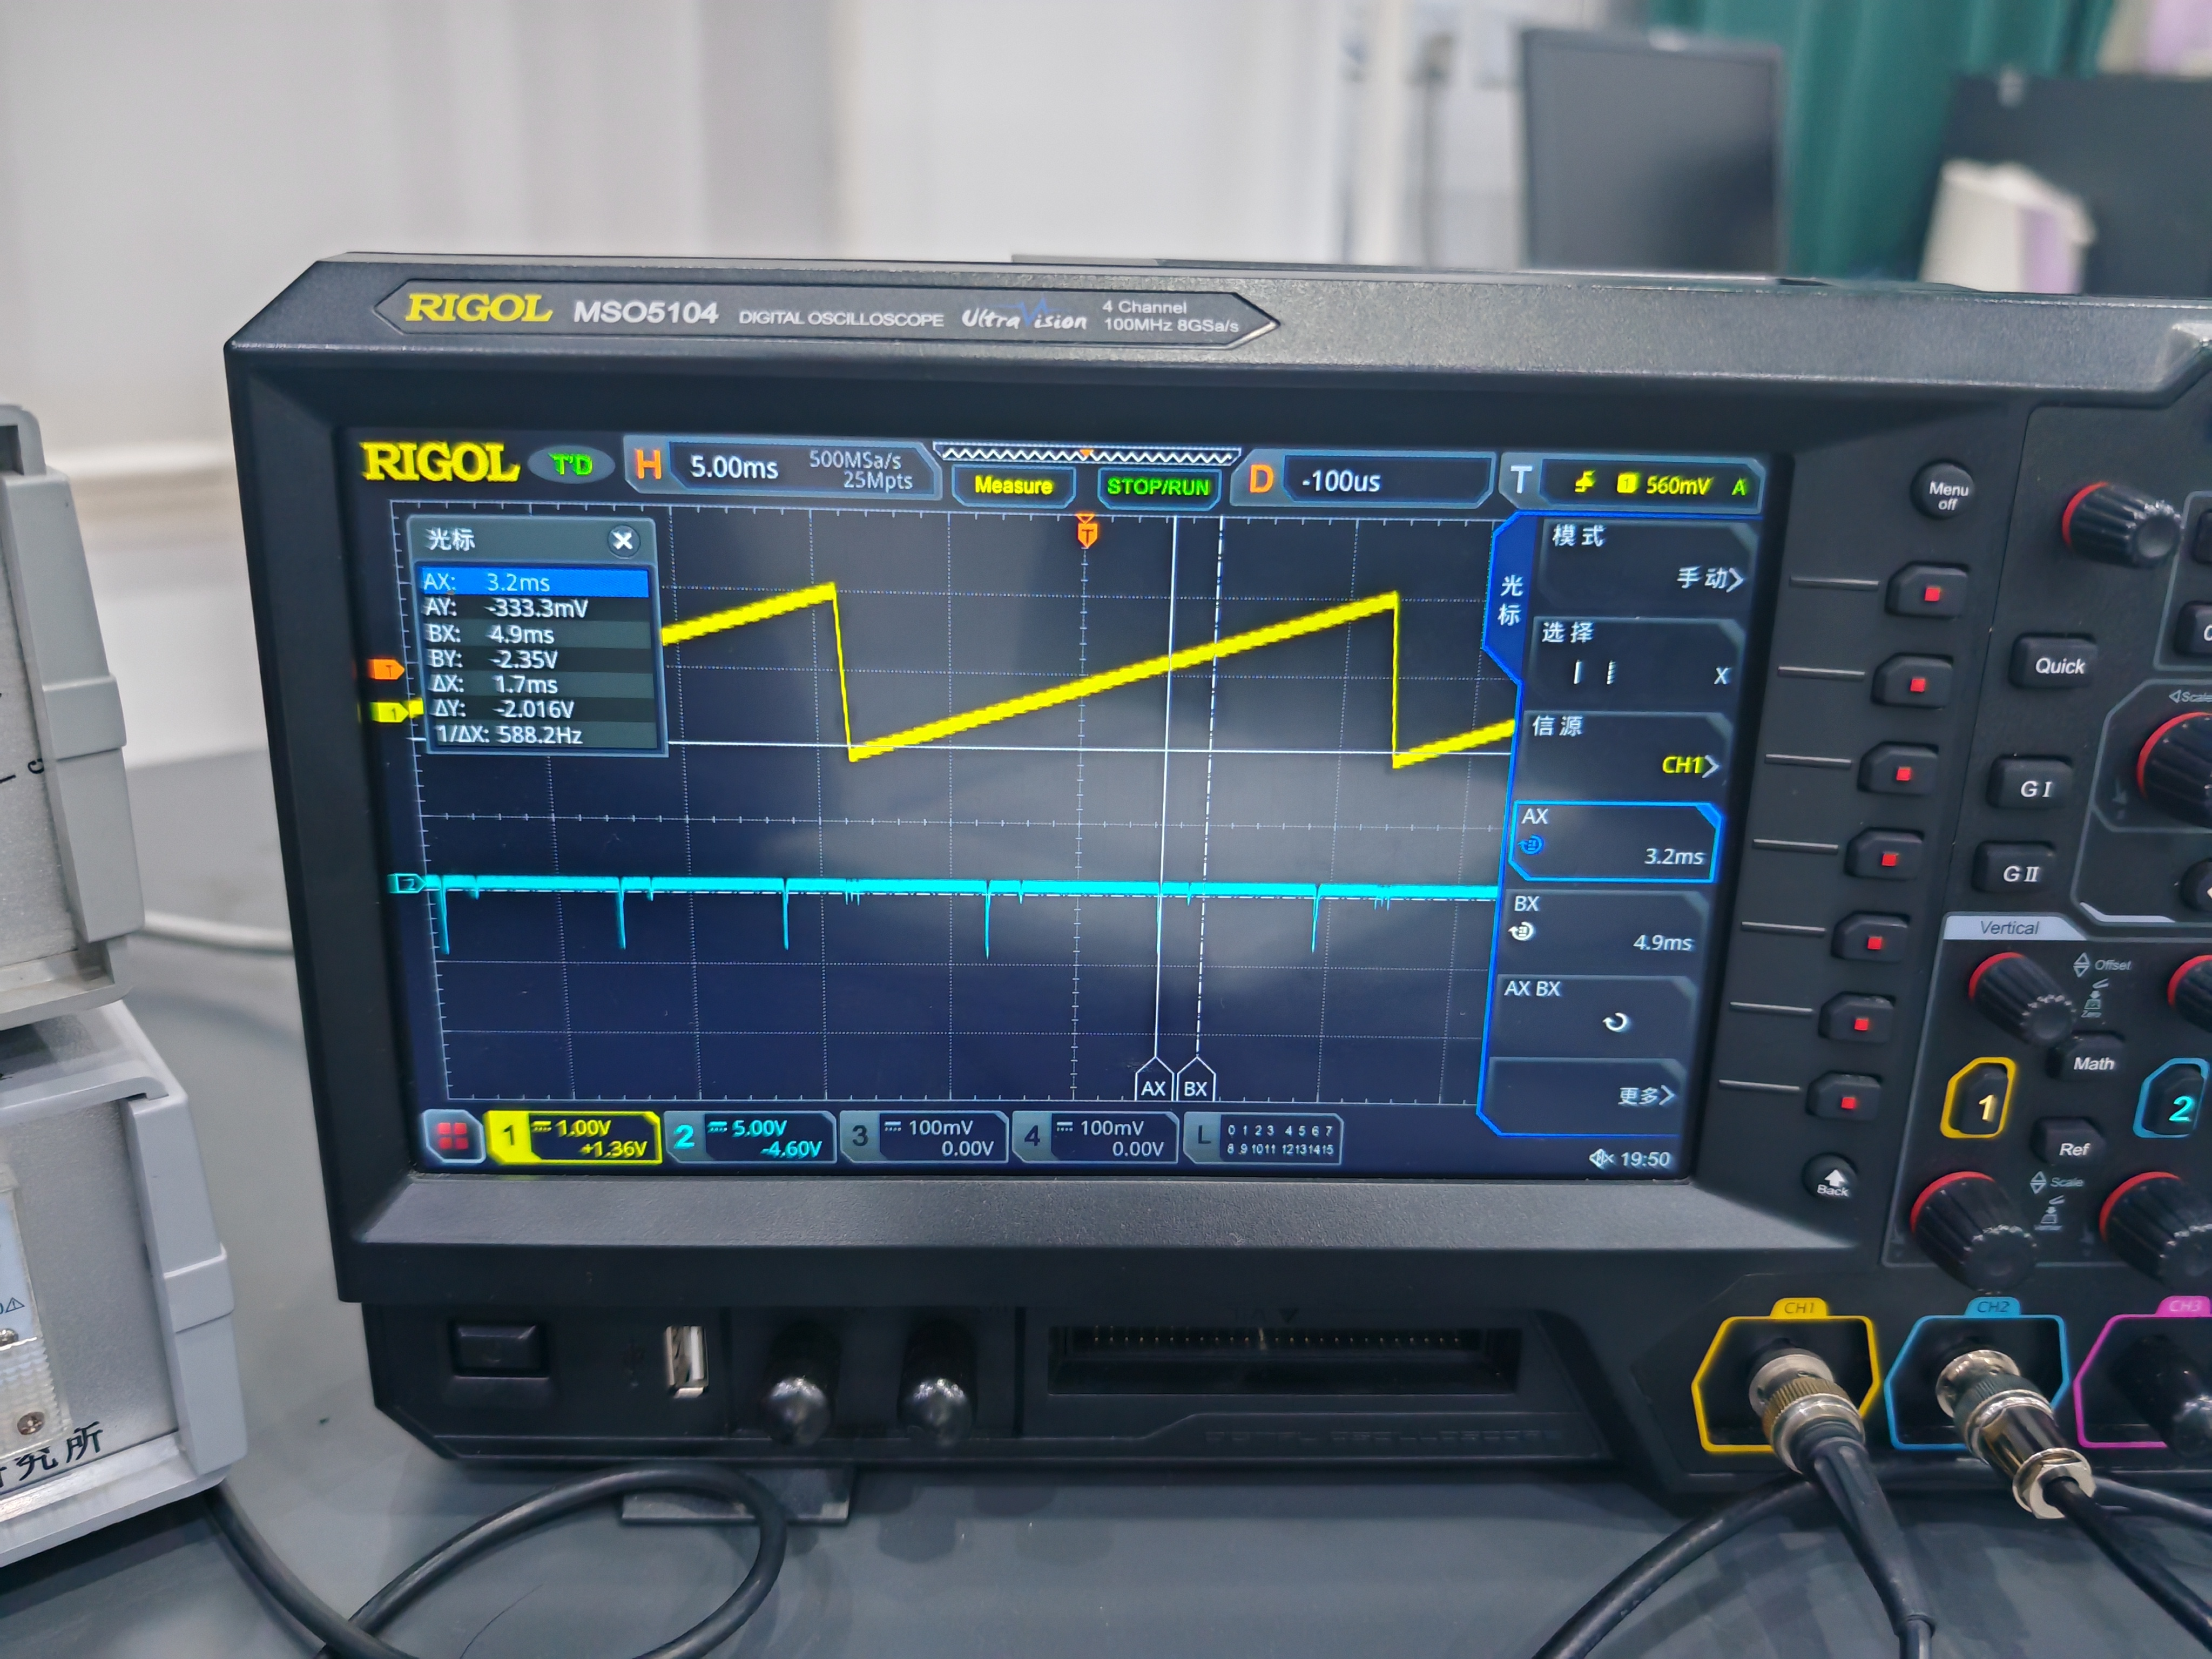
\includegraphics[width=\linewidth]{fig4.3_polarization_180.jpg}
    \subcaption{偏振片 $180^\circ$}
  \end{subfigure}\hfill
  \begin{subfigure}[t]{0.485\textwidth}
    \centering
    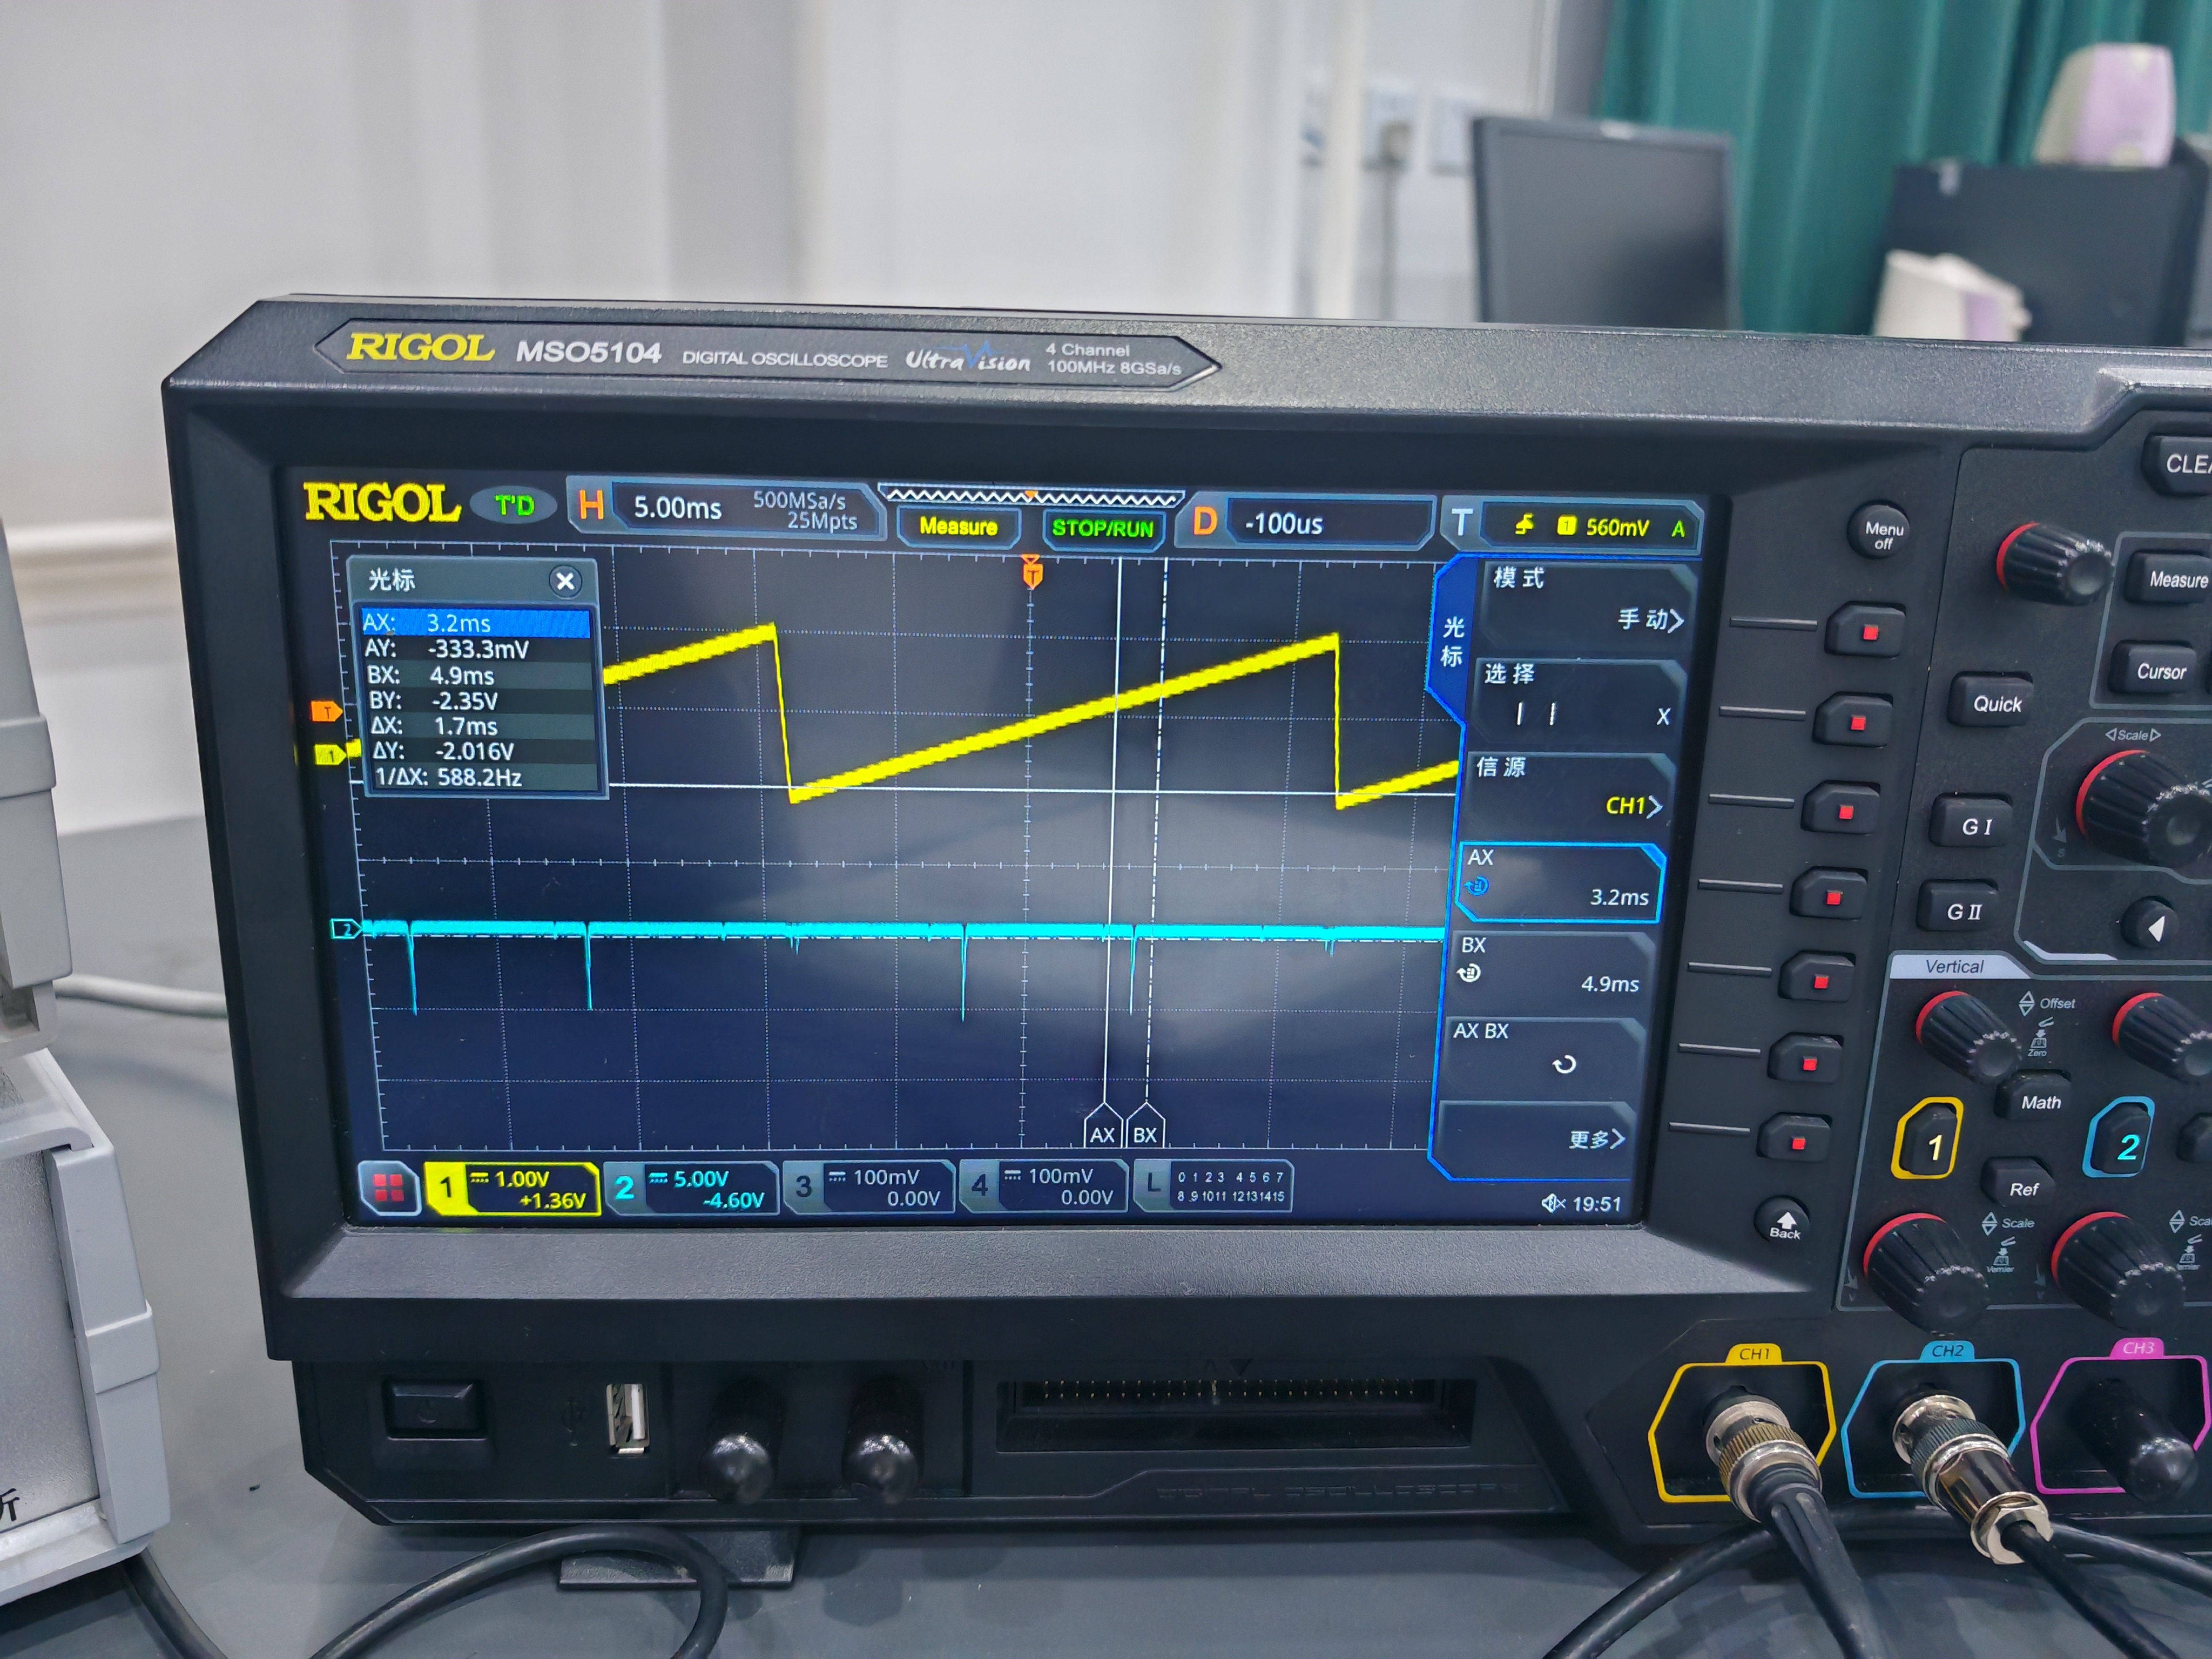
\includegraphics[width=\linewidth]{fig4.4_polarization_270.jpg}
    \subcaption{偏振片 $270^\circ$}
  \end{subfigure}
  \bicaption{固定石英晶片、旋转偏振片时两个分裂谱峰的示波器记录。}{Oscilloscope records of the two split peaks while the quartz plate is fixed and the polarizer is rotated.}
  \label{fig:polarization-scope}
\end{figure}

\begin{table}[H]
  \centering
  \caption{偏振片转角与两个分裂峰的电位幅度}
  \label{tab:polarization-result}
  \begin{tabular}{ccc}
    \toprule
    偏振片角度 $\theta$/degree & $U_1=|V_1|$/V & $U_2=|V_2|$/V \\
    \midrule
    0   & 2.983 & 2.433 \\
    15  & 2.866 & 2.766 \\
    30  & 2.666 & 3.083 \\
    45  & 2.516 & 3.100 \\
    60  & 2.350 & 3.366 \\
    75  & 2.333 & 3.666 \\
    90  & 2.346 & 3.650 \\
    105 & 2.566 & 3.416 \\
    120 & 2.716 & 3.000 \\
    135 & 2.800 & 2.600 \\
    150 & 2.833 & 2.383 \\
    165 & 3.083 & 2.350 \\
    180 & 3.116 & 2.400 \\
    \bottomrule
  \end{tabular}
\end{table}

图\ref{fig:polarization-data}给出了原始电位取幅度后的测量点及余弦平方拟合曲线。可以看出，第二个分裂峰的角度变化较接近理想曲线，而第一个分裂峰在 $0^\circ$--$90^\circ$ 区间的变化较平缓，数据点离散更明显。

\begin{figure}[H]
  \centering
  \begin{tikzpicture}
    \begin{axis}[
      width=0.94\linewidth,
      height=6.8cm,
      xmin=0,xmax=180,
      ymin=2.1,ymax=3.9,
      xtick={0,30,60,90,120,150,180},
      ytick={2.2,2.6,3.0,3.4,3.8},
      xlabel={偏振片角度 $\theta$/degree},
      ylabel={峰值幅度 $U$/V},
      grid=major,
      legend style={at={(0.02,0.98)},anchor=north west,font=\scriptsize},
      tick label style={font=\small},
      label style={font=\small}
    ]
      \addplot[only marks,mark=*,mark size=1.5pt,blue] coordinates {
        (0,2.983) (15,2.866) (30,2.666) (45,2.516) (60,2.350)
        (75,2.333) (90,2.346) (105,2.566) (120,2.716) (135,2.800)
        (150,2.833) (165,3.083) (180,3.116)
      };
      \addlegendentry{$U_1$ 测量值}
      \addplot[blue,thick,domain=0:180,samples=181] {2.682+0.353*cos(2*(x+13.6))};
      \addlegendentry{$U_1$ 拟合}
      \addplot[only marks,mark=square*,mark size=1.5pt,red] coordinates {
        (0,2.433) (15,2.766) (30,3.083) (45,3.100) (60,3.366)
        (75,3.666) (90,3.650) (105,3.416) (120,3.000) (135,2.600)
        (150,2.383) (165,2.350) (180,2.400)
      };
      \addlegendentry{$U_2$ 测量值}
      \addplot[red,thick,domain=0:180,samples=181] {2.983+0.636*cos(2*(x-76.3))};
      \addlegendentry{$U_2$ 拟合}
    \end{axis}
  \end{tikzpicture}
  \bicaption{偏振片转角与两个分裂峰幅度的测量值及余弦平方拟合。}{Measured amplitudes of the two split peaks and cosine-square fits versus polarizer angle.}
  \label{fig:polarization-data}
\end{figure}

对两个峰的幅度分别作 $U=C+A\cos[2(\theta-\theta_0)]$ 拟合，得到
\begin{align}
  U_1(\theta) &= 2.682+0.353\cos[2(\theta+13.6^\circ)]\ \si{\volt},
  &&R^2=0.942,\\
  U_2(\theta) &= 2.983+0.636\cos[2(\theta-76.3^\circ)]\ \si{\volt},
  &&R^2=0.958.
\end{align}
两个拟合曲线的极大方向相差约 $89.9^\circ$，接近正交偏振所要求的 $90^\circ$。两个峰幅度的 Pearson 相关系数为 $r=-0.940$，说明一个峰增强时另一个峰总体减弱，也支持两分裂模具有近似正交的偏振方向。
剩余偏差仍可能来自示波器读出的原始电位包含零线偏置、探测器暗电平和背景信号。严格来说，理论关系应作用于扣除背景后的峰值变化，测得电位更接近
\[
  U_i^{\mathrm{meas}}=U_{i,0}+k_i I_i(\theta),
\]
而本处理直接采用 $|V_i|$，会把 $U_{i,0}$ 和增益 $k_i$ 的影响混入偏振变化。其次，石英晶片的光轴、激光束和偏振片轴线未必完全对准，实际输出可能含有椭圆偏振或两个正交分量的串扰。

因此，$89.9^\circ$ 的极大方向差和 $r=-0.940$ 均支持两个分裂模近似正交偏振。改进时仍应先记录无光背景和示波器零线，用峰值相对基线的变化量代替 $|V_i|$；同时对每个角度重复测量并取平均，固定垂直档位和扫描参数，校准偏振片零点，并将非理想模型 $U_i^{\mathrm{meas}}=U_{i,0}+A_i\cos^2(\theta-\theta_i)$ 或其正弦形式直接用于拟合。

\subsection{实验五：石英晶片转角与两峰频差}

\textbf{频率换算与散点结果。}设左、右峰时间分别为 $t_{\mathrm{left}}$、$t_{\mathrm{right}}$，则本组标定关系为
\begin{equation}
 \Delta t=t_{\mathrm{right}}-t_{\mathrm{left}},\qquad
 \Delta\nu_{\mathrm{obs}}
 =\frac{\nu_{\mathrm{FSR}}}{T}\Delta t
 =\left(\SI{423.33}{\mega\hertz\per\milli\second}\right)\Delta t.
 \label{eq:quartz-scale}
\end{equation}
晶片垂直时示数为 $2.2^\circ$，故相对该位置的机械转角为 $\beta=\alpha-2.2^\circ$；作图保留原始示数 $\alpha$。
完整的排序数据及换算结果列于表\ref{tab:quartz-angle-raw}，散点见 Fig.~\ref{fig:quartz-angle}。纵轴表示所选两谱峰的频率间隔，不是激光的绝对光频率；低角度区域的小峰间距仅作如实展示。

\begin{figure}[H]
 \centering
 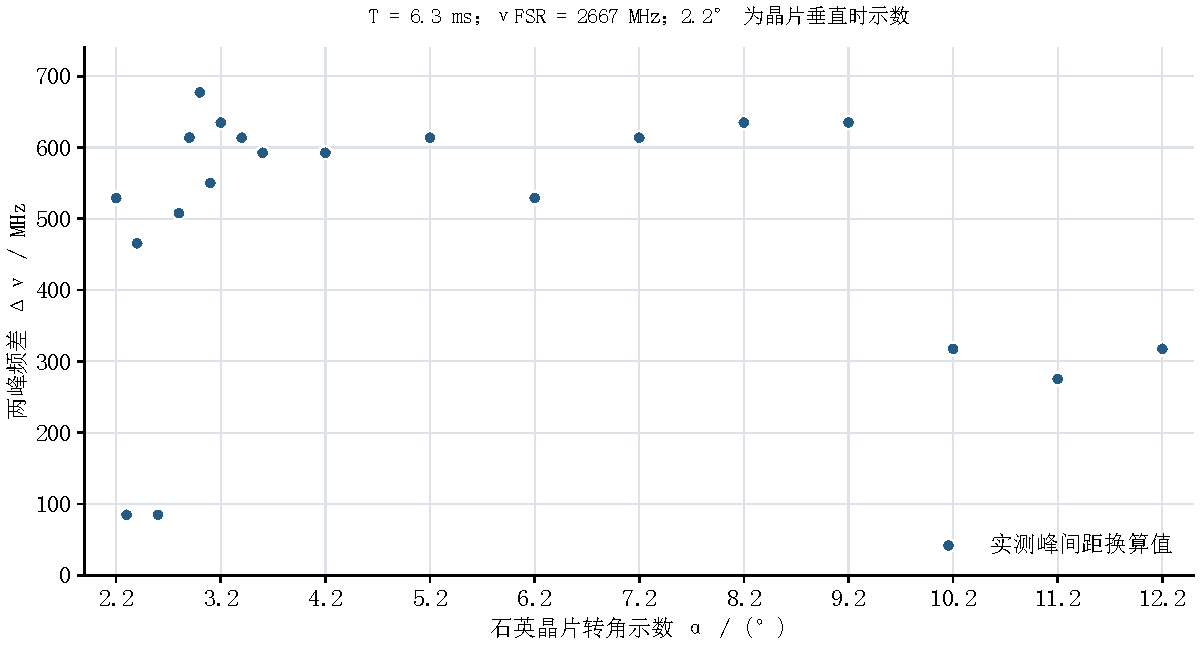
\includegraphics[width=0.8\linewidth]{figures/quartz_angle_scatter.pdf}
 \bicaption{石英晶片转角示数与两峰频差的实测散点。}
 {Measured peak-frequency separation versus quartz-plate angle reading.}
 \label{fig:quartz-angle}
\end{figure}

\textbf{锯齿状走势。}关注主要频差分支，$2.8^\circ$--$3.0^\circ$ 的频差由 \SI{508.0}{\mega\hertz} 升至 \SI{677.3}{\mega\hertz}，在 $3.1^\circ$ 回落到 \SI{550.3}{\mega\hertz}；$6.2^\circ$--$9.2^\circ$ 从 \SI{529.2}{\mega\hertz} 总体升到 \SI{635.0}{\mega\hertz}，随后 $10.2^\circ$ 降至 \SI{317.5}{\mega\hertz}。这些分段升高、回落和再次升高构成了类似锯齿的非单调走势。下降发生的精确角度只能限定在相邻采样点之间。

\textbf{物理解释与偏振关系。}按讲义的双折射近似，改变晶轴与光束夹角 $\vartheta$ 会改变非常光的有效折射率和两偏振分量的光程差，
\begin{equation}
 \delta(\vartheta)=h_{\mathrm{eff}}(\vartheta)
 [n_{e,\mathrm{eff}}(\vartheta)-n_o],\qquad
 \Delta\nu_b(\vartheta)\simeq \frac{\nu}{L_{\mathrm{opt}}}\delta(\vartheta).
 \label{eq:quartz-birefringence}
\end{equation}
其中 $h_{\mathrm{eff}}$ 为晶片内有效传播长度，$L_{\mathrm{opt}}$ 为激光腔单程光程，$\nu$ 为光频率；$\Delta\nu_b$ 是跟踪同一纵模级次时的双折射频移。该近似说明单个分支随角度移动的原因，并不直接预言一次连续转动必然产生理想锯齿。有关研究也显示，腔内相位延迟会改变两偏振纵模序列的相对位置，实际振荡模式还受模竞争影响\cite{liu2021}。

若示波器上实际选取的谱峰随角度改变而切换纵模级次，所读频差可定性表示为
\begin{equation}
 \Delta\nu_{\mathrm{obs}}(\alpha)
 \simeq \left|m(\alpha)\Delta\nu_{\mathrm{cav}}-\Delta\nu_b(\alpha)\right|,
 \label{eq:quartz-branch}
\end{equation}
其中 $\Delta\nu_{\mathrm{cav}}$ 是激光腔的纵模间隔，$m$ 是所选两峰的级次差。固定 $m$ 时频差沿一条分支变化；谱峰跨越、增益选择或模竞争改变可见峰和配对关系时，读数可能转入另一分支，表现为回落或折返。这为本组锯齿状走势提供了一个可能解释。由于记录只有每个角度的两个峰位，未连续标识峰的偏振身份和纵模序号，尚不能断定具体哪次回落就是模式跳变，也不能求出 $m$。

与此同时，在图中可以发现在靠近垂直位置的方位出现了较低的双峰间隔，对于原始图像可以视为单峰分裂成两个接近的小峰且该组没有出现其他峰。这个现象可能是由于实验过程中，o光和e光出现了耦合现象，在越远离垂直位置的地方越难看到相关现象。

\subsection{误差来源与改进建议}

实验频率间隔、出光带宽和偏振峰值均依赖示波器读数，主要测量限制如下。

\begin{enumerate}
  \item \textbf{扫描非线性与 PZT 滞回。}式\eqref{eq:scale}把示波器横轴近似视为线性频率轴，而压电陶瓷存在滞回和蠕变。可分别记录正、反向扫描，并利用每个自由光谱区的重复峰作分段标定或低阶多项式校正。
  \item \textbf{光路失调与峰宽增加。}激光束、干涉仪光轴和接收面不完全同轴会降低峰值并增大半高宽，影响峰位和分辨极限。应先用反射光斑重合完成粗调，再以峰值最大、峰宽最小为判据微调，并重复测量峰位。
  \item \textbf{热漂移和腔长漂移。}激光器、PZT 与电子学系统预热不足会使模谱随时间移动。应在仪器稳定后采集数据，固定扫描幅度和偏置电压，并在每组测量前后重新核验自由光谱区。
  \item \textbf{螺旋测微器调节与模式判别。}调节过程中可能发生模式跳变，单凭某一时刻的光斑或峰列容易误判。应在目标状态附近往返微调，同时记录观察屏图样与示波器峰列，并对同一模式重复取点。
  \item \textbf{出光边界的判定。}左右边界处的谱线强度逐渐减弱，消失点受噪声、峰宽和示波器读数分辨率影响。应统一边界判据，在同一频率标定下重复读取 $t_R$、$t_L$，并记录判据对应的背景水平。
  \item \textbf{偏振片零点和角度读数。}偏振片安装零点、刻度分辨率和手动转动误差会使拟合得到的极大方向发生偏移。应先校准零点，采用相同转动方向逐点测量，并在 $0^\circ$、$90^\circ$、$180^\circ$ 附近增加重复点。
  \item \textbf{峰值电位读数与峰形重叠。}两个分裂峰间距有限，峰宽、噪声和光标位置会影响峰值判断；示波器通道极性还会使峰形表现为负值。应固定垂直档位和零线，用同一峰值判据读取 $V_1$、$V_2$，并保留原始有符号电位后再取幅度。
  \item \textbf{光强漂移和探测器线性。}激光输出功率、光路耦合和探测器增益随时间变化会使两峰幅度和不再恒定。应在同一组测量中尽快完成角度扫描，记录总幅度作为漂移监视量，并确认探测器工作在线性范围内。
\end{enumerate}

\section{结论和建议}

本实验用扫描干涉仪完成了 He-Ne 激光纵、横模及出光带宽测量，并由纵模间隔反算管长。两组管长测量给出纵模频差平均值 \SI{677.86}{\mega\hertz}，管长为 \SI{221.3}{\milli\metre}，与尺量值的相对偏差为 \SI{0.32}{\percent}；$\mathrm{TEM}_{00}$、$\mathrm{TEM}_{01}$ 的纵模频差分别为 \SI{495.79}{\mega\hertz}、\SI{481.64}{\mega\hertz}，$\mathrm{TEM}_{01}$ 横模频差为 \SI{150.79}{\mega\hertz}，与观察屏上的光斑形态相符。三次出光带宽的平均值为 \SI{1103.34}{\mega\hertz}。

旋转偏振片时两个分裂峰幅度互补，极大方向相差约 $89.9^\circ$，说明两峰近似正交偏振。晶片转角的20组数据呈分段升降的锯齿状走势，$9.2^\circ$--$10.2^\circ$ 间频差由 \SI{635.0}{\mega\hertz} 降至 \SI{317.5}{\mega\hertz}；双折射引起的谱线移动和纵模分支变化可作定性解释，但尚不足以确定严格周期。主要误差来自峰位和带宽边界读数、扫描非线性、PZT 滞回、模式跳变及偏振片角度误差；可通过正反向扫描、局部加密采样、统一判据和重复测量改进。

\renewcommand{\refname}{六、参考文献}
\begin{thebibliography}{9}
  \bibitem{guide} 北京师范大学近代物理实验室．He-Ne 激光的纵横模分析和模分裂实验讲义[实验讲义]．北京：北京师范大学，2020．
  \bibitem{zhou} 周炳琨，高以智，陈家骅，等．激光原理[M]．北京：国防工业出版社，2000．
  \bibitem{liu2021} 刘维新，唐宁，马龙行，高克凡，孙明哲．Zeeman双频激光器频率分裂与纵模间隔变动一致性分析[J]．物理学报，2021，70(7)：074204．DOI：\href{https://doi.org/10.7498/aps.70.20200607}{10.7498/aps.70.20200607}．
\end{thebibliography}

\clearpage
\appendix
\renewcommand{\thetable}{A\arabic{table}}
\setcounter{table}{0}
\section*{附录 A\quad 实验原始数据}

\begin{table}[H]
  \centering
  \caption{实验一第一组峰位与逐差数据}
  \label{tab:exp1-raw}
  \begin{tabular}{lrrrrrr}
    \toprule
    记录量 & 1 & 2 & 3 & 4 & 5 & 6 \\
    \midrule
    峰位 $t_i$/ms & -3.85 & -1.60 & 4.55 & 6.55 & 12.20 & 14.00 \\
    选定峰差 $\delta t_i$/ms & 2.25 & 2.00 & 1.80 & -- & -- & -- \\
    重复间隔 $\delta T_i$/ms & 8.40 & 8.15 & 7.65 & 7.45 & -- & -- \\
    \bottomrule
  \end{tabular}
\end{table}

\begin{table}[H]
  \centering
  \caption{实验一第二组峰位与逐差数据}
  \begin{tabular}{lrrrrrr}
    \toprule
    记录量 & 1 & 2 & 3 & 4 & 5 & 6 \\
    \midrule
    峰位 $t_i$/ms & -4.75 & -2.55 & 3.60 & 5.55 & 11.10 & 12.90 \\
    选定峰差 $\delta t_i$/ms & 2.20 & 1.95 & 1.80 & -- & -- & -- \\
    重复间隔 $\delta T_i$/ms & 8.35 & 8.10 & 7.50 & 7.35 & -- & -- \\
    \bottomrule
  \end{tabular}
\end{table}

\begin{table}[H]
  \centering
  \caption{实验二 $\mathrm{TEM}_{00}$ 与 $\mathrm{TEM}_{01}$ 模谱峰位}
  \begin{tabular}{lrrrrrr}
    \toprule
    $\mathrm{TEM}_{00}$ 记录量 & 1 & 2 & 3 & 4 & 5 & 6 \\
    \midrule
    峰位 $t_i$/ms & -6.35 & -4.80 & 2.00 & 3.35 & 9.40 & 10.65 \\
    纵模峰差 $\delta t_i$/ms & 1.55 & 1.35 & 1.25 & -- & -- & -- \\
    重复间隔 $\delta T_i$/ms & 8.35 & 8.15 & 7.40 & 7.30 & -- & -- \\
    \bottomrule
  \end{tabular}
  \par\medskip
  \setlength{\tabcolsep}{8pt}
  \begin{tabular}{crrrrr}
    \toprule
    $\mathrm{TEM}_{01}$ 组次 & $t_1$/ms & $t_2$/ms & $t_3$/ms & $t_2-t_1$/ms & $t_3-t_2$/ms \\
    \midrule
    1 & -7.79 & 0.74 & 8.25 & 8.53 & 7.51 \\
    2 & -7.29 & 1.19 & 8.64 & 8.48 & 7.45 \\
    3 & -6.16 & 2.14 & 9.50 & 8.30 & 7.36 \\
    4 & -5.71 & 2.55 & 9.86 & 8.26 & 7.31 \\
    \bottomrule
  \end{tabular}
  \par\medskip
  \begin{tabular}{lccc}
    \toprule
    派生间隔 & 1 & 2 & 3 \\
    \midrule
    横模 $\delta t_i$/ms & 0.50 & 0.45 & 0.39 \\
    纵模 $\delta t_i$/ms & 1.63 & 1.40 & 1.25 \\
    \bottomrule
  \end{tabular}
\end{table}

\begin{table}[H]
  \centering
  \caption{实验三出光带宽原始数据与频率换算}
  \label{tab:bandwidth-raw}
  \setlength{\tabcolsep}{5pt}
  \begin{tabular}{c c c c c c c}
    \toprule
    次数 & $t_R$/ms & $t_L$/ms & $t_R-t_L$/ms & $T_{\mathrm{FSR}}$/ms & $\nu_{\mathrm{FSR}}$/MHz & $\Delta\nu_{\mathrm{out}}$/MHz \\
    \midrule
    1 & -0.90 & -3.60 & 2.70 & 6.325 & 2667 & 1138.48 \\
    2 & 4.55 & 2.05 & 2.50 & 6.325 & 2667 & 1054.15 \\
    3 & -17.25 & -19.90 & 2.65 & 6.325 & 2667 & 1117.40 \\
    平均 & -- & -- & -- & -- & -- & 1103.34 \\
    \bottomrule
  \end{tabular}
\end{table}

\begin{table}[H]
  \centering
  \caption{实验四偏振关系测量原始电位及幅度}
  \label{tab:polarization-raw}
  \setlength{\tabcolsep}{8pt}
  \begin{tabular}{ccccc}
    \toprule
    $\theta$/degree & $V_1$/V & $V_2$/V & $U_1=|V_1|$/V & $U_2=|V_2|$/V \\
    \midrule
    0   & -2.983 & -2.433 & 2.983 & 2.433 \\
    15  & -2.866 & -2.766 & 2.866 & 2.766 \\
    30  & -2.666 & -3.083 & 2.666 & 3.083 \\
    45  & -2.516 & -3.100 & 2.516 & 3.100 \\
    60  & -2.350 & -3.366 & 2.350 & 3.366 \\
    75  & -2.333 & -3.666 & 2.333 & 3.666 \\
    90  & -2.346 & -3.650 & 2.346 & 3.650 \\
    105 & -2.566 & -3.416 & 2.566 & 3.416 \\
    120 & -2.716 & -3.000 & 2.716 & 3.000 \\
    135 & -2.800 & -2.600 & 2.800 & 2.600 \\
    150 & -2.833 & -2.383 & 2.833 & 2.383 \\
    165 & -3.083 & -2.350 & 3.083 & 2.350 \\
    180 & -3.116 & -2.400 & 3.116 & 2.400 \\
    \bottomrule
  \end{tabular}
\end{table}

\begin{table}[H]
 \centering
 \caption{实验五晶片转角、原始峰位及频差（按角度升序）}
 \label{tab:quartz-angle-raw}
 \small
 \begin{tabular}{rrrrrr}
 \toprule
 工作簿行号 & $\alpha/(^\circ)$ & $t_{\mathrm{left}}/\mathrm{ms}$
 & $t_{\mathrm{right}}/\mathrm{ms}$ & $\Delta t/\mathrm{ms}$ & $\Delta\nu_{\mathrm{obs}}/\mathrm{MHz}$\\
 \midrule
 24 & 2.2 & -5.05 & -3.80 & 1.25 & 529.17\\
 35 & 2.3 & -4.60 & -4.40 & 0.20 & 84.67\\
 36 & 2.4 & 1.75 & 2.85 & 1.10 & 465.67\\
 37 & 2.6 & 2.10 & 2.30 & 0.20 & 84.67\\
 38 & 2.8 & -5.40 & -4.20 & 1.20 & 508.00\\
 39 & 2.9 & -4.90 & -3.45 & 1.45 & 613.83\\
 40 & 3.0 & -4.60 & -3.00 & 1.60 & 677.33\\
 41 & 3.1 & -5.50 & -4.20 & 1.30 & 550.33\\
 25 & 3.2 & -4.85 & -3.35 & 1.50 & 635.00\\
 42 & 3.4 & -4.65 & -3.20 & 1.45 & 613.83\\
 43 & 3.6 & -5.30 & -3.90 & 1.40 & 592.67\\
 26 & 4.2 & -3.20 & -1.80 & 1.40 & 592.67\\
 27 & 5.2 & -3.50 & -2.05 & 1.45 & 613.83\\
 28 & 6.2 & -4.35 & -3.10 & 1.25 & 529.17\\
 29 & 7.2 & -4.45 & -3.00 & 1.45 & 613.83\\
 30 & 8.2 & -4.90 & -3.40 & 1.50 & 635.00\\
 31 & 9.2 & -6.25 & -4.75 & 1.50 & 635.00\\
 32 & 10.2 & -4.90 & -4.15 & 0.75 & 317.50\\
 33 & 11.2 & 8.25 & 8.90 & 0.65 & 275.17\\
 34 & 12.2 & 1.90 & 2.65 & 0.75 & 317.50\\
 \bottomrule
 \end{tabular}
\end{table}
\end{document}
